\chapter{Solution Thermodynamics}\label{Chapter:SolutionThermodynamics}


   \begin{LearningObjectivesBlock}{Learning Objectives}
      Upon completion of this chapter, you will be able to
        \begin{enumerate}
           \item 
        \end{enumerate}
\medskip
     Recommended reading: Chapters 11-12 of \citet{SmithVanNess_Book}, 9-10 of \cite{Sandler_Book}, 6 \citet{Lue_Book}, 11 of \citet{Elliot_Book} or 5 of \citet{Atkins_Book}.
   \end{LearningObjectivesBlock}


%%%%%%%%%%%%%%%%%%%%%%%%%%%%%%%%%%%%%%%%%%%%%%%%%%%%%%%%%%%%%%%%%
\begin{comment}
   \begin{LearningObjectivesBlock}{Learning Objectives}
      Upon completion of this chapter, you will be able to
        \begin{enumerate}
           \item {\bf Knowledge:} Define, Name, Select, State 
           \item {\bf Comprehension:} Describe, Identify, Discuss
           \item {\bf Application:} Apply, Demonstrate, Employ, Sketch
           \item {\bf Analysis:} Analyse, Compare, Calculate, Solve
           \item {\bf Synthesis:} Determine, Formulate
           \item {\bf Evaluation:} Assess, Check, Estimate, Compare, Measure, Monitor
        \end{enumerate}
\end{comment}
%%%%%%%%%%%%%%%%%%%%%%%%%%%%%%%%%%%%%%%%%%%%%%%%%%%%%%%%%%%%%%%%%

%%%% ETOC
\localtableofcontents
   


%%% SUBSECTION
\section{Introduction}\label{Chapter:SolutionThermodynamics:Section:Introduction}
Vapour-liquid equilibrium of pure components and mixtures were the focus of study in Chapters~\ref{Chapter:VolumetricPropertiesPureSubstances}-\ref{Chapter:VLE}. In these chapters, equations of state were introduced to represent the $PVT$ behaviour of pure components in both vapour and liquid phases. From your readings, you may have noticed that EOS are largely applied, with relatively accuracy, to vapour phases, but rarely used to assess liquid phase behaviour. 

This is mainly due to the fact that EOS were originally (and cubic EOS in particular) to represent weak inter-molecular forces between gaseous molecules at relatively large distances (\ie {\it mean free path}). As pressure increases $\left(P\rightarrow \infty\right)$ and the distance between molecules tends to zero $\left(d\rightarrow 0\right)$, the accuracy of equations of state to predict $PVT$ behaviour also decreases, as the attractive and repulsive forces between molecules become stronger. 

Molecules in liquid phase are held together at close distances by strong attractive forces, however these forces are not strong enough to keep them in fixed positions (as inter-/intra-molecular forces in the solid phase) and the molecules are free to move past, slide over and collide with other molecules. A fraction of the molecules (mostly with higher energy) may be able to break such attractive forces and `escape' towards the vapour phase. 

Kinetic energy in gaseous molecules are larger than the attractive forces, leading to large distances between molecules and a tendency to occupy the whole volume of the system. The large kinetic energy in gaseous molecules also lead to continuous collisions between molecules and with the system (container) walls. During collisions, although total momentum is conserved, individual energies (and velocities) may decrease and molecules may move to a system with lower kinetic energy, \ie liquid phase.

\bigskip

In Chapter~\ref{Chapter:Introduction}, the concept of {\it mechanical} (\ie system at constant or uniform pressure) and {\it thermal} (from the Zeroth law) equilibrium were introduced. In order to define phase equilibria, we established (in Chapter~\ref{Chapter:ThermodynamicPropertiesPureFluids}) that an additional condition was necessary, {\it chemical equilibrium}, \ie equality of Gibbs free energy of all phases (Section~\ref{Chapter:ThermodynamicPropertiesPureFluids:Section:ClapeyronRelations}) for pure fluids. This concept can be extended for mixtures by using the definition of {\it chemical potential}, $\mu_{i}$ (Eqn.~\ref{Chapter:VLE:Eqn:ChemPotentialDef1b}),\index{Chemical potential}
         \begin{displaymath}
            \mu_{i} = \Partial[(nG)]{n_{i}}{T,P,n_{j\ne i}} \;\;\Longleftrightarrow\;\; \mu_{i} = \overline{G}_{i},
         \end{displaymath}
where $\overline{G}_{i}$ is the {\it partial molar Gibbs free energy}. This leads to the final phase equilibria condition in which {\it the chemical potential for each component at all coexisting phases are identical}, \ie 
         \begin{displaymath}
           \mfr[\mu]{i}{\alpha} = \mfr[\mu]{i}{\beta} = \cdots =  \mfr[\mu]{i}{j} = \cdots = \mfr[\mu]{i}{\mathcal{N}_{\mathcal{P}}}, \hspace{1.5cm} \forall i\in\{1,2,\cdots,\mathcal{C}\}\;\; \text{ and }\;\;\; \forall j\in\{\alpha,\beta,\cdots,\mathcal{N}_{\mathcal{P}}\}
         \end{displaymath}
         or for VLE systems:
         \begin{displaymath}
           \mfr[\mu]{i}{L} = \mfr[\mu]{i}{V},\;\;\;\forall i\in\{1,2,\cdots,\mathcal{C}\}
         \end{displaymath}

\medskip

The main assumptions for ideal gas behaviour assume that molecules of gas are massless particles with no interaction between them (\ie volume of the molecules is negligibly small compared with the volume occupied by the gas or simply the distance between gaseous molecules are often infinitely large, $d\rightarrow \infty$), except during elastic collisions over negligible duration. These conditions can only be met by fluids at sufficiently high temperature and relatively low pressure when large distances between molecules and high velocity overcome any interaction. The concept of ideality for liquids also exists and is based on the assumption that inter-molecular forces are the same between all molecules in solution. This assumption may be correct for pure non-polar substances (\ie in solutions with no major inter-/intra-molecular forces).

Thus, the aim of this Chapter is to define thermodynamic properties of real solutions based on properties of ideal solutions. Excess properties (Section~\ref{Chapter:VLE:Section:ExcessProperties}) plays a role similar to that of residual properties (Section~\ref{Chapter:ThermodynamicPropertiesPureFluids:Section:ResidualProperties}) for gases. In order to study solution properties at low to moderate pressures, {\it activity coefficient}, based on the definition of {\it fugacity}, is used. The {\it activity coefficient}, derived from the {\it excess Gibbs free energy}, is a measure of the extent of non-ideality of a real solution and helps describing phase equilibria of mixtures at low and moderate pressures.


%%% SECTION
\section{Fugacity}\label{Chapter:SolutionThermodynamics:Section:FugacitySection}\index{Fugacity}
\begin{subequations}
  A formal definition for {\it partial molar property} was introduced in Section~\ref{Chapter:VLE:Section:PartialMolarProperties} for an arbitrary extensive function $M$, Eqn.~\ref{Chapter:VLE:Eqn:PartialProperties2}. Such formulation was applied to the Gibbs free energy of a system with $n=n_{1}+n_{2}+\cdots+n_{\mathcal{C}}$ moles leading to the definition of the {\it chemical potential}, Eqns.~\ref{Chapter:VLE:Eqn:ChemPotentialDef1}-\ref{Chapter:VLE:Eqn:ChemPotentialDef1b},
  \begin{shaded}
     \begin{eqnarray}
       && dG = \Partial[G]{P}{T,n}dP + \Partial[G]{T}{P,n}dT + \underbrace{\Partial[G]{n}{T,P}}_{\mu}dn, \nonumber \\
       && \mu_{i} = \Partial[(nG)]{n_{i}}{T,P,n_{j\ne i}} \;\;\Longleftrightarrow\;\; \mu_{i} = \overline{G}_{i}, \nonumber
     \end{eqnarray}
  \end{shaded}
  \noindent For pure components,
  \begin{displaymath}
    G = n\mu \;\;\rightarrow \mu=\frc{G}{n}=\overline{g},
  \end{displaymath}
  where $\overline{g}$ is the molar Gibbs free energy. Using the Maxwell relation, Eqn.~\ref{Chapter:ThermodynamicPropertiesPureFluids:Eqn:MaxwellRelation7},
  \begin{eqnarray}
    && \Partial[G]{P}{T} = V = \Partial[n\mu]{P}{T} = n\Partial[\mu]{P}{T} \nonumber \\
    && \Partial[\mu]{P}{T} = \frc{V}{n} = \overline{v}\label{Chapter:SolutionThermodynamics:Eqn:fugacity1}
  \end{eqnarray}
  where $\underline{v}$ is the molar volume. For an ideal gas,
  \begin{displaymath}
     \Partial[\mu^{\text{ig}}]{P}{T} = \frc{RT}{P},
  \end{displaymath}
  where the superscript {\it ig} refers to ideal gas. This differential can be integrated as,
  \begin{equation}
    \mu^{\text{ig}} = RT\ln{P} + C(T),\label{Chapter:SolutionThermodynamics:Eqn:fugacity1a}
  \end{equation}
  where $C(T)$ is an integration constant. At limiting conditions, $P\rightarrow 0$ and $P\rightarrow\infty$, the chemical potential lies within $-\infty < \mu < +\infty$.
  \begin{shaded}
    \noindent For a fluid to be considered an ideal gas, pressure needs to be relatively low, thus we can use Eqn.~\ref{Chapter:SolutionThermodynamics:Eqn:fugacity1a} to represent the \underline{chemical potential of real fluids},
  \begin{equation}
    \mu = RT\ln{f} + C(T),\label{Chapter:SolutionThermodynamics:Eqn:fugacity1b}
  \end{equation}
  where $f$ is the {\it fugacity of a real gas}, \ie \blue{a representation of the pressure of an ideal gas that has the same chemical potential as the real gas.}
  \end{shaded}
  \noindent Since the {\it fugacity} has the \underline{units of pressure}, it is often referred as a `fictitious pressure'.  The definition of fugacity from Eqn.~\ref{Chapter:SolutionThermodynamics:Eqn:fugacity1b} is entirely general and can be readily extended to both liquids and solids. Now, replacing Eqn.~\ref{Chapter:SolutionThermodynamics:Eqn:fugacity1b} in the Maxwell relation, Eqn.~\ref{Chapter:ThermodynamicPropertiesPureFluids:Eqn:MaxwellRelation7}, at constant temperature,
  \begin{equation}
    RT\Partial[\left(\ln{f}\right)]{P}{T} = \overline{v}.\label{Chapter:SolutionThermodynamics:Eqn:fugacity1c}
  \end{equation}
  {\it Fugacity} can be obtained by integrating this equation holding $T$ constant. As pressure tends to zero (lower limit of the left-hand-side integration), the fluid behaves as an ideal gas. We can thus state that the fugacity of a pure component is equal to the pressure in the limit of zero pressure, \ie
      \begin{shaded}
        \begin{equation}
           \lim\limits_{P \rightarrow 0} \frc{f}{P} = 1.\label{Chapter:SolutionThermodynamics:Eqn:fugacity1d}
        \end{equation}
      \end{shaded}

  \noindent  In a \underline{mixture} containing $n$ moles of $\mathcal{C}$ chemical species, Eqn.~\ref{Chapter:SolutionThermodynamics:Eqn:fugacity1c} becomes,
      \begin{eqnarray}
        && RT\Partial[\left(\ln{f_{i}}\right)]{P}{T,n} = \overline{v}_{i},\;\;\;\;\forall i\in\left\{1,2,\cdots,\mathcal{C}\right\}\label{Chapter:SolutionThermodynamics:Eqn:fugacity1e1} \\
        && RT\Partial[\left(\ln{\overline{f}_{i}}\right)]{P}{T,n} = \overline{V}_{i},\label{Chapter:SolutionThermodynamics:Eqn:fugacity1e2}
      \end{eqnarray}
      where $f_{i}$ is the {\it fugacity of pure component $i$} and $\overline{f}_{i}$ is the {\it fugacity of component $i$ in the mixture}. $\overline{v}_{i}$ and $\overline{V}_{i}$ are the molar volume of pure component $i$ and, of component $i$ in the mixture. If we subtract Eqn.~\ref{Chapter:SolutionThermodynamics:Eqn:fugacity1e1} from \ref{Chapter:SolutionThermodynamics:Eqn:fugacity1e2} and integrate the result from $P'$ to $P$ at constant $T$,
      \begin{displaymath}
        RT\Partial[\left(\ln{\frc{\overline{f}_{i}}{f_{i}}}\right)]{P}{T,n} = \overline{V}_{i} - \overline{v}_{i} \;\;\Longrightarrow \;\;  RT\left[\left.\ln{\left(\frc{\overline{f}_{i}}{f_{i}}\right)}\right|_{P'}^{P}\right] = \int\limits_{P'}^{P}\left(\overline{V}_{i} - \overline{v}_{i}\right)dP
      \end{displaymath}
      Assuming that $P'$ tends to $0$,
      \begin{equation}
        RT\left[\ln{\left(\frc{\overline{f}_{i}}{f_{i}}\right)} - \lim\limits_{P'\rightarrow 0}\ln\left(\frc{\overline{f}_{i}}{f_{i}}\right)\right] = \int\limits_{0}^{P}\left(\overline{V}_{i} - \overline{v}_{i}\right)dP.\label{Chapter:SolutionThermodynamics:Eqn:fugacity1f}
      \end{equation}
      When $P'\rightarrow 0$
      \begin{displaymath}
        \begin{cases}
          f_{i} \rightarrow P', \\
          \overline{f}_{i} \rightarrow y_{i}P',
        \end{cases}
      \end{displaymath}
      and the limiting term in the previous equation becomes,
      \begin{displaymath}
        \lim\limits_{P'\rightarrow 0}\ln\left(\frc{\overline{f}_{i}}{f_{i}}\right) \rightarrow \ln{\left(\frc{y_{i}P'}{P'}\right)} = \ln{y_{i}}
      \end{displaymath}
      Thus Eqn.~\ref{Chapter:SolutionThermodynamics:Eqn:fugacity1f} becomes,
        \begin{displaymath}
          RT\left[\ln{\left(\frc{\overline{f}_{i}}{f_{i}}\right)} - \ln{y_{i}}\right] = \int\limits_{0}^{P}\left(\overline{V}_{i} - \overline{v}_{i}\right)dP
        \end{displaymath}
      \begin{shaded}
        \begin{equation}
           RT\ln{\left(\frc{\overline{f}_{i}}{y_{i}f_{i}}\right)} = \int\limits_{0}^{P}\left(\overline{V}_{i} - \overline{v}_{i}\right)dP. \label{Chapter:SolutionThermodynamics:Eqn:fugacity1g}
        \end{equation}
      \end{shaded}
  \noindent This expression relates fugacity of a pure component $i$ and the fugacity of the same component $i$ in a mixture with $\mathcal{C}$ chemical components during continuous change in pressure. The term in brackets in the left-hand side represents the ratio between partial pressures between real and ideal fluids in a mixture.

  \bigskip
        
      For an ideal mixture of ideal gases, the partial pressure of species $i$ is the fugacity of component $i$ in the mixture, \ie
         \begin{displaymath}
            \mfr[\overline{f}]{i}{V} = y_{i}P = P_{i}.
         \end{displaymath}
      Now, for an ideal mixture of real fluids,
         \begin{displaymath}
            \mfr[\overline{f}]{i}{L} = x_{i}\mfr[f]{i}{L},
         \end{displaymath}
      \ie the fugacity of a component in a mixture is a function of the fugacity of the pure component.
      \begin{shaded}
         An \underline{ideal solution} is a mixture in which,
        \begin{equation}
          \mfr[\overline{f}]{i}{V} = y_{i}P = P_{i}\;\;\;\text{ and }\;\;\; \mfr[\overline{f}]{i}{L} = x_{i}\mfr[f]{i}{L}\label{Chapter:SolutionThermodynamics:Eqn:fugacity2a}
        \end{equation}
        These expressions are called {\it Lewis-Randall rules} and they describe relations between phase compositions and fugacities.\index{Lewis-Randall rules|see {Solutions}}\index{Solutions!Lewis-Randall rules}
      \end{shaded}
      
\end{subequations}

      
%%% SECTION
\section{Activity and Activity Coefficient }\label{Chapter:SolutionThermodynamics:Section:ActivitySection}\index{Activity|see {Solutions}}\index{Solutions!Activity}\index{Activity coefficient|see {Solutions}}\index{Solutions!Activity coefficient}
   \begin{subequations}
      
      In a mixture with $\mathcal{C}$ chemical species in $n\;\left(= n_{1}+n_{2}+\cdots +n_{\mathcal{C}}\right)$ moles, the chemical potential of each component is (based on Eqn.~\ref{Chapter:SolutionThermodynamics:Eqn:fugacity1b}),
        \begin{displaymath}
           \mu_{i} = RT\ln{\overline{f}_{i}} + C_{i}(T).
        \end{displaymath}
      Let's consider a reference-state where a species $i$ of a multi-component system is pure at temperature $T$ and at reference-state pressure, $P_{\text{ref}}$,
        \begin{equation}
           \mu_{i} - \mu_{i}^{\circ} = RT\ln{\left(\frc{\overline{f}_{i}}{f_{i}^{\circ}}\right)},\label{Chapter:SolutionThermodynamics:Eqn:activity1a}
        \end{equation}
      where superscript $^{\circ}$ stands for {\it reference state}. 
        \begin{shaded}
           \noindent Now, we can define the term in brackets as the {\it activity} (dimensionless)
           \begin{equation}
              \frc{\overline{f}_{i}}{f_{i}^{\circ}} = a_{i}, \label{Chapter:SolutionThermodynamics:Eqn:activity1b}
           \end{equation}
           which `measures' the deviation from ideal behaviour.
        \end{shaded}
      \noindent Since $\mu^{\circ} = \overline{g}^{\circ}_{i}$, Eqn.~\ref{Chapter:SolutionThermodynamics:Eqn:activity1a} becomes
        \begin{equation}
           \mu_{i} = \overline{g}^{\circ}_{i} + RT\ln{a_{i}}\label{Chapter:SolutionThermodynamics:Eqn:activity1c}
        \end{equation}
      For an ideal solution, the {\it Lewis-Randall relation} can be used,\index{Solutions!Lewis-Randall rules}
        \begin{displaymath}
           a_{i} =  \frc{\overline{f}_{i}}{f_{i}^{\circ}} = \frc{y_{i}f_{i}}{f_{i}^{\circ}},
        \end{displaymath}
      where $f_{i}$ is the fugacity of pure component $i$ at $P$ and $T$, and $f_{i}^{\circ}$ is the fugacity of pure component $i$ at $T$ and the reference-pressure $P_{\text{ref}}$. Thus,
        \begin{displaymath}
           \mu_{i} = \overline{g}^{\circ}_{i} + RT\ln{\left( \frc{y_{i}f_{i}}{f_{i}^{\circ}}\right)}.
        \end{displaymath}

        \begin{shaded}
            \noindent For \underline{\it ideal solutions},
              \begin{equation}
                 \mu_{i} = \overline{g}^{\circ}_{i} + RT\ln{\left[\left(\frc{f_{i}}{P}\right)\left(\frc{P_{\text{ref}}}{f_{i}^{\circ}}\right)\frc{y_{i}P}{P_{\text{ref}}}\right]}.\label{Chapter:SolutionThermodynamics:Eqn:activity1d}
              \end{equation}
            If component $i$ behaves as an \underline{\it ideal gas} at both $\left(T,P\right)$ and $\left(T,P_{\text{ref}}\right)$, thus $\frc{f_{i}}{P} = \frc{f_{i}^{\circ}}{P_{\text{ref}}}=1$ and Eqn.~\ref{Chapter:SolutionThermodynamics:Eqn:activity1d} becomes
              \begin{equation}
                 \mu_{i} = \overline{g}^{\circ}_{i} + RT\ln{\frc{y_{i}P}{P_{\text{ref}}}}.\label{Chapter:SolutionThermodynamics:Eqn:activity1e}
              \end{equation}
             This expression allows the calculation of the chemical potential of the vapour phase in a mixture subjected to a change in pressure based on composition and temperature. {\it Molar Gibbs energy at reference conditions}, $\overline{g}^{\circ}_{i}$, for several chemical species are often tabulated and can be found in any chemical engineering handbook.
             
        \noindent Finally, we can now define the \underline{\blue{activity coefficient}}, $\gamma_{i}$, as
          \begin{equation}
              a_{i} = \frc{y_{i}f_{i}}{f_{i}^{\circ}}\;\;\;\;\Rightarrow \;\;\;\; \gamma_{i} = \frc{a_{i}}{y_{i}} = \frc{f_{i}}{f_{i}^{\circ}}\label{Chapter:SolutionThermodynamics:Eqn:activity1f}
          \end{equation}
         And for solutions,
          \begin{equation}
              \gamma_{i} = \frc{\overline{f}_{i}}{x_{i}f_{i}}\label{Chapter:SolutionThermodynamics:Eqn:activity1g}
          \end{equation}
         The{\it activity coefficient} takes into account non-idealities in the liquid phase. Now, we can properly define the \underline{Raoult's law} (Section~\ref{Chapter:VLE:Section:RaoultsLaw}) at low pressure,\index{Solutions!Raoult's law}
          \begin{equation}
               \gamma_{i} = \frc{\overline{f}_{i}}{x_{i}f_{i}} = \frc{y_{i}P}{x_{i}f_{i}}=\frc{y_{i}P}{x_{i}P_{i}^{\text{sat}}} \;\;\;\Longrightarrow \;\;\;\ x_{i}\gamma_{i}P_{i}^{\text{sat}} = y_{i}P \label{Chapter:SolutionThermodynamics:Eqn:RaoultLaw}
          \end{equation}
          Equation~\ref{Chapter:SolutionThermodynamics:Eqn:RaoultLaw} is the general form for Raoult's law. If the solution is ideal, $\gamma_{i}=1$, Eqn.~\ref{Chapter:VLE:Eqn:RaoultLaw} is recovered.

      \end{shaded}       
%
   \end{subequations}
      
%%% SECTION
\section{Henry's Law}\label{Chapter:SolutionThermodynamics:Section:HenryLaw}\index{Solutions!Henry's law}
Now that the concepts of fugacity and activity coefficient were introduced, we can return to the special VLE condition in which the solute is very diluted in the mixture (Section~\ref{Chapter:VLE:Section:HenryLaw}). In such cases, the fugacity of a very dilute chemical species in a liquid mixture (\eg dissolved gases or solid of limited solubility) is experimentally found to be a linear function of its low composition (\ie mole fraction)\footnote{It is clear that the division in the limiting term,
  \begin{displaymath}
    \lim\limits_{x_{i}\rightarrow 0}\frc{\overline{f_{i}}}{x_{i}}
  \end{displaymath}
  is undetermined as $f_{i}=0\text{ when }x_{i}\rightarrow 0$, \ie at infinite dilution of a solute $i$ in solution, the fugacity of this component is null. In order to solve this mathematical problem, we can use the L'H\^opital rule (see Appendix~\ref{Appendix:lHopital}) which states that for a limit,
         \begin{displaymath}
                 \lim\limits_{x\rightarrow a}\frc{f(x)}{g(x)},
         \end{displaymath}
         if the numerator and denominator are finite at $a$, and $g(a)=0$, then
         \begin{displaymath}
                 \lim\limits_{x\rightarrow a}\frc{f(x)}{g(x)} =  \lim\limits_{x\rightarrow a}\frc{f'(a)}{g'(a)}.
         \end{displaymath}
         Therefore, the limiting dilution case can be solved as
         \begin{displaymath}
                 \lim\limits_{x_{i}\rightarrow 0}\frc{\overline{f_{i}}}{x_{i}} = \left(\frc{d \overline{f_{i}}}{d x_{i}}\right)_{x_{i}=0}.
         \end{displaymath}
}, \ie   
      \begin{eqnarray}
        && \lim\limits_{x_{i}\rightarrow 0}\frc{\overline{f_{i}}}{x_{i}} = \left(\frc{d \overline{f_{i}}}{d x_{i}}\right)_{x_{i}=0}  \equiv \mathcal{H}_{i}, \nonumber \\
        && \mfr[\overline{f}]{i}{L}(T,P,x) = x_{i}\mathcal{H}_{i}(T,P)\;\;\;\;\text{ as } x_{i}\rightarrow 0.
      \end{eqnarray}      
This proportionality constant, $\mathcal{H}$, is called {\it Henry's law constant}, and is dependent on the solute-solvent pair, temperature and pressure. This experimentally-defined constant was first introduced in Eqn.~\ref{Chapter:VLE:Eqn:HenryLaw} as, in equilibrium conditions (at $P$, $T$ and $n$ constants), $\mfr[\overline{f}]{i}{V}=\mfr[\overline{f}]{i}{L}$,
         \begin{shaded}
           \begin{displaymath}
             P_{i} = y_{i}P = x_{i}\mathcal{H}_{i},
           \end{displaymath}
           with $\mfr[\overline{f}]{i}{V}=y_{i}P$.
        \end{shaded}
%
%%%%%
%%%%%  COMMENTS
%%%%%
\begin{comment}      

\begin{table}[h]
   \begin{center}
      \begin{tabular}{l c l l l}
          \hline
             {\bf Components}   & {\bf Basis}  & {\bf Standard-state}   & {\bf Activity}        & {\bf Limits} \\
          \hdashline
             Solid or liquid    &              &  Pure                  & $a=1$                 &              \\
          \hdashline
             Solvent            &   Raoult     &  Pure solvent          & $a=\frc{P}{P_{\text{ref}}}$,  & $\gamma\rightarrow 1\text{ as } x\rightarrow 1$ \\
                                &              &                        & $a=\gamma x$          &  (pure solvent) \\
          \hdashline
             Solute             & Henry        & (1) hypothetical state of& $a=\frc{P}{\mathcal{H}}$,& $\gamma\rightarrow 1\text{ as } x\rightarrow 0$ \\
                                &              & pure solute            & $a=\gamma x$          &                                     \\
          \hdashline
                                &              & (2) hypothetical state of& $a=\gamma\frc{m}{m^{\circ}}$& $\gamma\rightarrow 1\text{ as } m\rightarrow 0$ \\
                                &              & solute at molality $m$   &                     &                                     \\
         \hline 
       \end{tabular}
       \caption{Standard states for activity \citep[extracted from][]{Atkins_Book}.}\label{Chapter:SolutionThermodynamics:Table:StandarStateActivity}
   \end{center}
\end{table}
\end{comment}

%%% SECTION
\section{Gibbs-Duhem Equation}\label{Chapter:SolutionThermodynamics:Section:GibbsDuhem}\index{Gibbs-Duhem equation|see {Solutions}}\index{Solutions!Gibbs-Duhem equation}
   \begin{subequations}
%
       In Section~\ref{Chapter:VLE:Section:PartialMolarProperties}, the concept of \underline{\it partial molar property} of species $i$ in solution was defined as\index{Partial molar properties}
         \begin{displaymath}
            \overline{M}_{i} = \Partial[(nM)]{n_{i}}{T,P,n_{j\ne i}},
         \end{displaymath}
        \ie the change of the total property $nM$ of a mixture of $\mathcal{C}$ species resulting from the addition at constant $T$ and $P$ of infinitesimal amount of species $i$ to a prescribed amount of solution.  It is important to bear in mind that {\it partial molar property} of a substance is different from {\it molar property} of the same substance in a pure state at the same $T$ and $P$. This is due to inter-/intra-molecular forces that imposes interactions between species in solution.
\medskip

      Equation~\ref{Chapter:VLE:Eqn:PartialProperties2} is a general expression for the change of any extensive property, $M$
         \begin{displaymath}
            d(nM) = n\Partial[M]{P}{T,x}dP + n\Partial[M]{T}{P,x}dT + \summation[\overline{M}_{i}dn_{i}]{i}{}.
         \end{displaymath}
      Mole fraction of a species $i$ was also introduced in Section~\ref{Chapter:VLE:Section:Compositions} as,
         \begin{displaymath}
            x_{i} = \frc{n_{i}}{n} \;\;\Rightarrow\;\; n_{i} = x_{i}n,
         \end{displaymath}
      Applying {\it derivative of a product} rule (Appendix~\ref{Appendix_Calculus:Section:BasicDerivationIntegration}) on $n_{i}$,
         \begin{displaymath}
             dn_{i} = x_{i}dn + n dx_{i},
         \end{displaymath}
      and for the total property $(nM)$,
         \begin{displaymath}
             d(nM) = n d M + M dn.
         \end{displaymath}
      Replacing these expressions in Eqn.~\ref{Chapter:VLE:Eqn:PartialProperties2},
        \begin{displaymath}
           n d M + M d n = n \Partial[M]{T}{P,x}dT + n\Partial[M]{P}{T,x}dP + \summation[\overline{M}_{i}\left(x_{i}dn + ndx_{i}\right)]{i}{}
        \end{displaymath}
      Rearranging this expression,
        \begin{equation}
           \underbrace{\left[dM - \Partial[M]{T}{P,x}dT - \Partial[M]{P}{T,x}dP - \summation[\overline{M}_{i}dx_{i}]{i}{}\right]}_{A}n + \underbrace{\left[M-\summation[\overline{M}_{i}x_{i}]{i}{}\right]}_{B}dn = 0.\label{Chapter:SolutionThermodynamics:Eqn:GibbsDuhem1a}
        \end{equation}
      Equation~\ref{Chapter:SolutionThermodynamics:Eqn:GibbsDuhem1a} is valid for any arbitrary values of $n$ and $dn$, therefore $n$ and $dn$ should be independent of each other. Therefore, this expression is only true if the coefficients $A$ and $B$ are zero, \ie
          \begin{eqnarray}
              A &=& dM - \Partial[M]{T}{P,x}dT - \Partial[M]{P}{T,x}dP - \summation[\overline{M}_{i}dx_{i}]{i}{} = 0 \nonumber \\
              dM &=& \Partial[M]{T}{P,x}dT + \Partial[M]{P}{T,x}dP + \summation[\overline{M}_{i}dx_{i}]{i}{}, \label{Chapter:SolutionThermodynamics:Eqn:GibbsDuhem1b}
          \end{eqnarray}
      and
          \begin{eqnarray}
              B &=& M-\summation[\overline{M}_{i}x_{i}]{i}{} = 0 \nonumber \\
              M &=& \summation[\overline{M}_{i}x_{i}]{i}{}\label{Chapter:SolutionThermodynamics:Eqn:GibbsDuhem1c} \\
             \text{as } nM = n\summation[\overline{M}_{i}x_{i}]{i}{} &\Rightarrow& dM = \summation[x_{i}d \overline{M}_{i}]{i}{} + \summation[\overline{M}_{i}dx_{i}]{i}{}\label{Chapter:SolutionThermodynamics:Eqn:GibbsDuhem1d}
          \end{eqnarray}
      Replacing Eqn.~\ref{Chapter:SolutionThermodynamics:Eqn:GibbsDuhem1d} in Eqn.~\ref{Chapter:SolutionThermodynamics:Eqn:GibbsDuhem1b} leads to the \blue{\it Gibbs-Duhem Equation (GDE)},
          \begin{shaded}
             \begin{equation}
                 \Partial[M]{T}{P,x}dT + \Partial[M]{P}{T,x}dP - \summation[x_{i}d\overline{M}_{i}]{i}{} = 0.\label{Chapter:SolutionThermodynamics:Eqn:GibbsDuhem1e}
             \end{equation}
             The \blue{GDE} must be satisfied for all changes in $P$, $T$ and $\overline{M}_{i}$. For changes at constant temperature and pressure conditions, the GDE becomes
               \begin{equation}
                   \summation[x_{i}d\overline{M}_{i}]{i}{} = 0.\label{Chapter:SolutionThermodynamics:Eqn:GibbsDuhem1f}
               \end{equation}
             Or taking any arbitrary species $j$,
               \begin{equation}
                   \summation[x_{i}\frc{d\overline{M}_{i}}{dx_{j}}]{i}{} = 0, \;\;\;\text{ at constant } T\text{ and } P.\label{Chapter:SolutionThermodynamics:Eqn:GibbsDuhem1g}
               \end{equation}
             Equations~\ref{Chapter:SolutionThermodynamics:Eqn:GibbsDuhem1f}-\ref{Chapter:SolutionThermodynamics:Eqn:GibbsDuhem1g} imply that partial molar properties of various species, $\overline{M}_{i}$, are \underline{not} independent. 

             \noindent Some key-properties,
               \begin{displaymath}
                   \begin{cases}
                       \lim\limits_{x_{i}\rightarrow 0}\overline{M}_{i} = \overline{M}_{i}^{\infty} & \text{\ie at infinite dilutions;} \\
                       \lim\limits_{x_{i}\rightarrow 1}\overline{M}_{i} = M_{i}                   & \text{ \ie nearly pure chemical species.} 
                   \end{cases}
               \end{displaymath}
          \end{shaded}
%
   \end{subequations}


      
%%% SECTION
\section{Partial Molar Properties in Binary Solutions}\label{Chapter:SolutionThermodynamics:PMP_Binary}\index{Partial molar properties}
   \begin{subequations}
%
       In a mixture with $n$ moles, we can define the {\it isothermal molar property change of mixing}, $\Delta M_{\text{mix}}$ as,\index{Molar property change of mixing}
          \begin{eqnarray}
              \Delta M_{\text{mix}}(T,P) & = & M(T,P) - \summation[x_{i}M_{i}(T,P)]{i}{} \nonumber \\
                                      &=& \underbrace{\summation[\overline{M}_{i}x_{i}]{i}{}}_{\text{from Eqn.~\ref{Chapter:SolutionThermodynamics:Eqn:GibbsDuhem1c}}} - \summation[x_{i}M_{i}]{i}{} \nonumber \\
                                      &=& \summation[x_{i}\left(\overline{M}_{i}-M_{i}\right)]{i}{}.\label{Chapter:SolutionThermodynamics:Eqn:GibbsDuhem1h}
          \end{eqnarray}
       \begin{shaded}
          \nonindent In a \underline{binary system} (from Eqn.~\ref{Chapter:SolutionThermodynamics:Eqn:GibbsDuhem1c}),
          \begin{equation}
              M = \overline{M}_{1} x_{1} + \overline{M}_{2} x_{2},\;\;\;\;\;\left(\text{at constant }P \text{ and } T\right),\label{Chapter:SolutionThermodynamics:Eqn:GibbsDuhem1i}
          \end{equation}
       \end{shaded}
       \noindent and using the {\it derivative of a product} rule on $M$,
          \begin{displaymath}
              dM = \left(x_{1}d\overline{M}_{1} + \overline{M}_{1}dx_{1}\right) + \left(x_{2}d\overline{M}_{2} + \overline{M}_{2}dx_{2}\right), 
          \end{displaymath}
      applying GDE (Eqn.~\ref{Chapter:SolutionThermodynamics:Eqn:GibbsDuhem1f}) in this expression, and using 
          \begin{displaymath}
             \summation[x_{i}]{i}{}=1\;\;\Leftrightarrow\;\; x_{1}+x_{2}=1\;\;\Rightarrow\;\;\; dx_{1}=-dx_{2},
          \end{displaymath}
      leads to 
          \begin{eqnarray}
             && \cancel{\red{x_{1}d\overline{M}_{1}}} + \overline{M}_{1}dx_{1} + \cancelto{\red{=0 \text{ (due to GDE, Eqn.~\ref{Chapter:SolutionThermodynamics:Eqn:GibbsDuhem1f})}}}{\red{x_{2}d\overline{M}_{2}}} - \overline{M}_{2}dx_{1} = dM \nonumber \\
             && dM = \overline{M}_{1}dx_{1} - \overline{M}_{2}dx_{1} \nonumber \\
             && \frc{dM}{dx_{1}} = \overline{M}_{1} - \overline{M}_{2} \label{Chapter:SolutionThermodynamics:Eqn:GibbsDuhem1j}
          \end{eqnarray}
          \begin{shaded}
             Using Eqn.~\ref{Chapter:SolutionThermodynamics:Eqn:GibbsDuhem1i} in Eqn.~\ref{Chapter:SolutionThermodynamics:Eqn:GibbsDuhem1j},
               \begin{eqnarray}
                  && \frc{dM}{dx_{1}} = \overline{M}_{1} - \left(\frc{M-\overline{M}_{1}x_{1}}{x_{2}}\right) \nonumber \\
                 && x_{2}\frc{dM}{dx_{1}} =  \underbrace{x_{2}\overline{M}_{1}}_{\left(1-x_{1}\right)\overline{M}_{1}} - M + \overline{M}_{1}x_{1} \nonumber
               \end{eqnarray}
               \begin{equation}
                 \begin{cases}
                    \overline{M}_{1} = M + x_{2}\frc{dM}{dx_{1}},\\% \label{Chapter:SolutionThermodynamics:Eqn:GibbsDuhem1k} \\
                    \overline{M}_{2} = M - x_{1}\frc{dM}{dx_{1}} \label{Chapter:SolutionThermodynamics:Eqn:GibbsDuhem1k}
                 \end{cases}
              \end{equation}
            In binary solutions, the partial molar properties can be easily calculated from these two  expressions as a function of composition at constant $T$ and $P$. %From the GDE,
              \begin{eqnarray}
                   && x_{1}d\overline{M}_{1} + x_{2}d\overline{M}_{2} = 0 \;\;\;\;\;\blue{\times\frc{1}{dx_{1}}} \nonumber \\
                   && x_{1}\frc{d\overline{M}_{1}}{dx_{1}} + x_{2}\frc{d\overline{M}_{2}}{dx_{1}} = 0 \;\;\;\;\;\blue{\times\frc{1}{x_{1}}}\nonumber \\ %\label{Chapter:SolutionThermodynamics:Eqn:GibbsDuhem1l} \\
                   && \frc{d\overline{M}_{1}}{dx_{1}} + \frc{x_{2}}{x_{1}}\frc{d\overline{M}_{2}}{dx_{1}} = 0. \label{Chapter:SolutionThermodynamics:Eqn:GibbsDuhem1l} 
              \end{eqnarray}
          \end{shaded}
 %
   \end{subequations}
      
%%% SECTION
\section{Ideal Gas Mixture Model}\label{Chapter:SolutionThermodynamics:IGM}\index{Gases!Mixture}
   \begin{subequations}
%
     Since Module~\ref{Section:01}, we have used the equation of state for {\it ideal gases},
     \begin{displaymath}
        PV = nRT \;\;\;\Rightarrow\;\;\; P\overline{v} = RT
     \end{displaymath}
     In an {\it ideal gas mixture} (igm), the EOS has a similar format,
     \begin{equation}
       PV^{\text{igm}} = \underbrace{\left(n_{1}+n_{2}+\cdots+n_{\mathcal{C}}\right)}_{N\text{ moles}}RT = \left(\summation[n_{i}]{i=1}{\mathcal{C}}\right)RT = NRT.\label{Chapter:SolutionThermodynamics:Eqn:IGM1} 
     \end{equation}
     The internal energy of the gaseous mixture, $U^{\text{igm}}$, is just the summation of the internal energies of the individual components of the mixture,
     \begin{equation}
       U^{\text{igm}}(T,N) = \summation[n_{i}\overline{u}_{i}^{\text{ig}}(T)]{i=1}{\mathcal{C}},\label{Chapter:SolutionThermodynamics:Eqn:IGM2} 
     \end{equation}
     where $\overline{u}_{i}^{\text{ig}}=\frac{U_{i}^{\text{ig}}}{n_{i}}$ is the molar internal energy.We can change the notation on Eqns.~\ref{Chapter:SolutionThermodynamics:Eqn:IGM1}-\ref{Chapter:SolutionThermodynamics:Eqn:IGM2} to replace the number of moles by molar fraction, $y_{i}$, of the gas mixture, and to obtain the {\it partial molar internal energy}, $\overline{U}_{i}^{\text{igm}}(T,y)$
     \begin{equation}
       \overline{U}_{i}^{\text{igm}}(T,y) = \Partial[U^{\text{igm}}(T,N)]{n_{i}}{T,P,n_{j\ne i}} = \left[\frc{\partial\summation[n_{j}\overline{u}_{j}^{\text{ig}}(T)]{j=1}{\mathcal{C}}}{\partial n_{i}}\right]_{T,P,n_{j\ne i}}  = \overline{u}_{i}^{\text{ig}}(T)\label{Chapter:SolutionThermodynamics:Eqn:IGM3}
     \end{equation} 
     This expression indicates that the partial molar internal energy of species $i$ in an ideal gas mixture at a given tempereature is equal to the pure component molar internal energy of that component behaving as an ideal gas at the same temperature. We can also obtain the {\it partial molar volume}, $\overline{V}_{i}^{\text{igm}}$, with the same conclusion,
     \begin{equation}
       \overline{V}_{i}^{\text{igm}}(T,P,y) = \Partial[V^{\text{igm}}(T,P,N)]{n_{i}}{T,P,n_{j\ne i}} = \left[\frc{\partial\summation[n_{j} \frc{RT}{P}]{j=1}{\mathcal{C}}}{\partial n_{i}}\right]_{T,P,n_{j\ne i}} = \frc{RT}{P} = \overline{v}_{i}^{\text{ig}}(T,P).\label{Chapter:SolutionThermodynamics:Eqn:IGM4}
     \end{equation}
     \medskip

     The partial pressure of species $i$ in a gas mixture, $P_{i}$ (see Dalton's law in Section~\ref{Section:04:RaoultsLaw}), is defined for both ideal and real gas mixtures as
     \begin{displaymath}
       P_{i} = y_{i}P,
     \end{displaymath}
     and for an ideal gas mixture,
     \begin{equation}
       P_{i}^{\text{igm}}(N,T,V,y) = \frc{n_{i}}{\summation[n_{j}]{j=1}{\mathcal{C}}}P = \frc{n_{i}}{\summation[n_{j}]{j=1}{\mathcal{C}}}\left[\summation[n_{j}\frc{RT}{V}]{j=1}{\mathcal{C}}\right] = \frc{n_{i}RT}{V} = P^{\text{ig}}\left(n_{i},V,T\right),\label{Chapter:SolutionThermodynamics:Eqn:IGM4}
     \end{equation}
     \ie for ideal gas mixtures, the partial pressure of species $i$ is equal to the pressure that would be exerted if the same number of moles of that species, $n_{i}$, alone were contained in the same volume, $V$, at $T$ and $P$. 
\medskip

     As there is {\bf no} effective inter-/intra-molecular interactions in an ideal gas mixture, the effect on each species of the mixture at constant $T$ and $P$ is equivalent to:
     \begin{itemize}
       \item reducing the pressure from $P$ to $P_{i}$, or;
       \item expanding each gas from its initial volume $V_{i}=n_{i}RT/P$ to $V=\summation[n_{i}RT/P]{}{}$.
     \end{itemize}
     Thus using the entropy relations below for ideal gases\footnote{These relations have not been derived in this Notes, but can be obtained assuming $S=S(T,P)$ and $S=S(T,V)$, definitions of coefficients of thermal expansion, $\beta$, and isothermal compressibility, $\kappa$, Eqn.~\ref{Mod02_Compressibilityexpansivity}, and Maxwell relations.},
       \begin{displaymath}
           dS =
         \begin{cases}
              C_{p}d\left(\ln{T}\right) - Rd\left(\ln{P}\right), \\
              C_{v}d\left(\ln{T}\right) + Rd\left(\ln{V}\right),
         \end{cases}          
     \end{displaymath}
     leading to (assuming constant $T$),
       \begin{displaymath}
           \overline{S}_{i}^{\text{igm}}(T,P,y) - \overline{s}_{i}^{\text{ig}}(T,P) =
         \begin{cases}
              -R\ln{\frc{P_{i}}{P}} = -R\ln{y_{i}}\;\;\;\text{ or }, \\
               R\ln{\frc{V}{V_{i}}} = R\ln{\frc{\summation[n_{j}RT/P]{j}{}}{n_{i}RT/P}} = -R\ln{y_{i}},
         \end{cases}          
     \end{displaymath}
     for the whole mixture, the molar entropy change of mixing, $\Delta_{\text{mix}}\overline{S}^{\text{igm}}$ (see Eqn.~\ref{Chapter:SolutionThermodynamics:Eqn:GibbsDuhem1h}) can be obtained from
     \begin{displaymath}
          \Delta_{\text{mix}}S^{\text{igm}} = \summation[n_{i}\left(\overline{S}_{i}^{\text{igm}}(T,P,y) - \overline{s}_{i}^{\text{ig}}(T,P) \right) ]{i=1}{\mathcal{C}} = -R\summation[n_{i}\ln{y_{i}}]{i=1}{\mathcal{C}}.
     \end{displaymath}
     If this expression is divided by the total number of moles, $\summation[n_{j}]{j=1}{\mathcal{C}}$,
     \begin{equation}
       \Delta_{\text{mix}}\overline{s}^{\text{igm}} = - R \summation[y_{i}\ln{y_{i}}]{i=1}{\mathcal{C}}.
     \end{equation}
\medskip
  
     \noindent With volume, internal energy and entropy change of mixing, partial molar properties of other thermodynamic potentials can be readily obtained. For enthalpy,
     \begin{eqnarray}
          && \overline{H}_{i}^{\text{igm}}(T,P,y) = \overline{h}_{i}^{\text{ig}}(T,P) \nonumber \\
          && \overline{H}^{\text{igm}}(T,P,y) = \summation[y_{i}\overline{h}_{i}^{\text{ig}}(T,P)]{i=1}{\mathcal{C}},
     \end{eqnarray}
     and for Gibbs free energy from $G=H-TS$,
     \begin{eqnarray}
       \overline{G}_{i}^{\text{igm}}(T,P,y) &=& \overline{H}_{i}^{\text{igm}}(T,P,y) - T\overline{S}_{i}^{\text{igm}}(T,P,y) \nonumber \\
                                        &=& \overline{h}_{i}^{\text{ig}}(T,P) - T\left[ \overline{s}_{i}^{\text{ig}}(T,P) - R\ln{y_{i}}\right] \nonumber \\
                                        &=& \overline{g}_{i}^{\text{ig}}(T,P) + RT\ln{y_{i}},
     \end{eqnarray}
     and the Gibbs free energy change of mixing,
     \begin{eqnarray}
        \Delta_{\text{mix}}\overline{g}_{i}^{\text{igm}} &=& \summation[y_{i}\left(\overline{G}_{i}^{\text{igm}}(T,P,y)-\overline{g}_{i}^{\text{ig}}(T,P)\right)]{i=1}{\mathcal{C}} \nonumber \\
                                        &=& RT\summation[y_{i}\ln{y_{i}}]{i=1}{\mathcal{C}} \nonumber 
     \end{eqnarray}


 \begin{table}\scriptsize
     \begin{tabular}{ | c | c | c | c |}%\scriptsize
 \hline
        {\bf Property}    &   {\bf Partial Molar}   &  {\bf Change of Mixing}                    &  {\bf Molar Property} \\
                          &   {\bf Property}        &  $\left(\mathbf{\Delta_{\text{mix}}}\right)$  &                       \\
 \hline
            Volume        &   $\overline{V}_{i}^{\text{igm}}(T,y) = \overline{v}_{i}^{\text{ig}}(T)$ & $\Delta_{\text{mix}} \overline{v}^{\text{igm}}=0 $ & $\overline{v}^{\text{igm}}(T,P,y) = \summation[y_{i}\overline{v}_{i}^{\text{ig}}(T,P)]{}{}$ \\
         Internal Energy  &   $\overline{U}_{i}^{\text{igm}}(T,y) = \overline{u}_{i}^{\text{ig}}(T)$ & $\Delta_{\text{mix}} \overline{u}^{\text{igm}}=0 $ & $\overline{u}^{\text{igm}}(T,y) = \summation[y_{i}\overline{u}_{i}^{\text{ig}}(T)]{}{}$ \\
         Enthalpy         &   $\overline{H}_{i}^{\text{igm}}(T,y) = \overline{h}_{i}^{\text{ig}}(T)$ & $\Delta_{\text{mix}} \overline{h}^{\text{igm}}=0 $ & $\overline{h}^{\text{igm}}(T,P,y) = \summation[y_{i}\overline{h}_{i}^{\text{ig}}(T,P)]{}{}$ \\
         Entropy          &   $\overline{S}_{i}^{\text{igm}}(T,P,y) = \overline{s}_{i}^{\text{ig}}(T,P)-R\ln{y_{i}}$ & $\Delta_{\text{mix}} \overline{s}^{\text{igm}}=-R\summation[y_{i}\ln{y_{i}}]{}{}$ & $\overline{s}^{\text{igm}}(T,P,y) = \summation[y_{i}\overline{s}_{i}^{\text{ig}}(T,P)]{}{}-R\summation[y_{i}\ln{y_{i}}]{}{}$ \\
         Gibbs Energy     &   $\overline{G}_{i}^{\text{igm}}(T,P,y) = \overline{g}_{i}^{\text{ig}}(T,P)+RT\ln{y_{i}}$ & $\Delta_{\text{mix}} \overline{g}^{\text{igm}}=-RT\summation[y_{i}\ln{y_{i}}]{}{}$ & $\overline{g}^{\text{igm}}(T,P,y) = \summation[y_{i}\overline{g}_{i}^{\text{ig}}(T,P)]{}{} + RT\summation[y_{i}\ln{y_{i}}]{}{}$ \\
         Helmholtz Energy &   $\overline{A}_{i}^{\text{igm}}(T,P,y) = \overline{a}_{i}^{\text{ig}}(T,P)+RT\ln{y_{i}}$ & $\Delta_{\text{mix}} \overline{a}^{\text{igm}}=-RT\summation[y_{i}\ln{y_{i}}]{}{}$ & $\overline{a}^{\text{igm}}(T,P,y) = \summation[y_{i}\overline{a}_{i}^{\text{ig}}(T,P)]{}{} + RT\summation[y_{i}\ln{y_{i}}]{}{}$ \\ 
 \hline
     \end{tabular}
     \caption{Properties of ideal gas mixtures \citep[extracted from][]{Sandler_Book}.}\label{Chapter:SolutionThermodynamics:Eqn:TableIGM}  
 \end{table}
     
     Partial molar properties, molar properties and change of mixing of molar properties for the main thermodynamic functions are summarised in Table~\ref{Chapter:SolutionThermodynamics:Eqn:TableIGM}.
%
   \end{subequations}


      
%%% SECTION
\section{Fugacity Coefficient of Species in Mixtures}\label{Chapter:SolutionThermodynamics:FugacityCoefficient}
   \begin{subequations}
%
      In  Section~\ref{Chapter:SolutionThermodynamics:FugacitySection} (Eqn.~\ref{Chapter:SolutionThermodynamics:Eqn:fugacity1b}), a formal definition of fugacity was introduced,
       \begin{displaymath}
          \mu_{i}= RT\ln{\overline{f}_{i}} + C_{i}(T),
       \end{displaymath}
       where $\overline{f}_{i}$ is the fugacity of species $i$ in the mixture. For pure fluids, the \blue{fugacity coefficient}, $\phi$, can be defined as,
       \begin{equation}
         \phi = \frc{f}{P}.
       \end{equation}
       For pure ideal gases, $f^{\text{ig}}=P$ (obtained from the definition of fugacity $\lim\limits_{P\rightarrow 0}\frac{f}{P}=1$) and $\phi^{\text{ig}}=1.$
       \begin{shaded}
         \noindent The definition of fugacity coefficient can be extended to {\it real gas mixtures} and {\it real liquid solutions} as,
         \begin{eqnarray}
           \mfr[\phi]{i}{V} &=& \frc{\mfr[\overline{f}]{i}{V}}{y_{i}P}\;\;\text{ and, }\\
           \mfr[\phi]{i}{L} &=& \frc{\mfr[\overline{f}]{i}{L}}{x_{i}P_{i}^{\text{sat}}}.
         \end{eqnarray}
       \end{shaded}

\medskip
       For a single component in a closed system behaving as an ideal gas, the fundamental thermodynamic relation is valid,
         \begin{displaymath}
            dG = VdP - SdT,
         \end{displaymath}
         at constant temperature, a pure gas $i$, this relation reduces to,
         \begin{displaymath}
            dG_{i}^{\text{ig}} = V_{i}^{\text{ig}}dP = RT\frc{dP}{P} = RTd\ln{P}.
         \end{displaymath}
         Integrating this expression leads to,
         \begin{displaymath}
             G_{i}^{\text{ig}} = RT\ln{P} + C_{i}(T),
         \end{displaymath}
         where $C_{i}$ is an integration constant. With the same procedure, but now for a real fluid, we can obtain a relation between the Gibbs free energy of species $i$ and the fugacity at constant $T$,
         \begin{displaymath} 
             G_{i} = RT\ln{f_{i}} + C_{i}(T).
         \end{displaymath}
         Subtracting these expressions results in the {\it residual Gibbs free energy},
         \begin{equation}
            G_{i}^{R} = G_{i} - G_{i}^{\text{ig}} = RT\ln{f_{i}}{P} = RT\ln{\phi_{i}}.
         \end{equation}
         Using the Gibbs free energy generating function, Eqn.~\ref{Mod03_ResidualProperties_GeneratingGibbsFunction3}, %$\frc{G^{R}}{RT} =  \int\limits_{0}^{P}\left(Z-1\right)\frc{dP}{P}$,
         \begin{equation}
            \ln{\phi_{i}} = \int\limits_{0}^{P}\left(Z-1\right)\frc{dP}{P}
         \end{equation}
\bigskip

         \noindent During phase change from saturated liquid to saturated vapour,
         \begin{equation}
            \mfr[G]{i}{V} - \mfr[G]{i}{L} = RT\ln{\frc{\mfr[f]{i}{V}}{\mfr[f]{i}{L}}},\label{Chapter:SolutionThermodynamics:Eqn:FugacityCoeff1}
         \end{equation}
         however, from Section~\ref{Section:03:ClapeyronRelations}, we studied that during phase transition \blue{$dG=0$}, \ie
         \begin{displaymath}
            \mfr[G]{i}{V} - \mfr[G]{i}{L} = 0 = RT\ln{\frc{\mfr[f]{i}{V}}{\mfr[f]{i}{L}}}
         \end{displaymath}
         \begin{shaded}
            \begin{equation}
               \mfr[f]{i}{V} = \mfr[f]{i}{L} = \mfr[f]{i}{\text{sat}} \;\;\text{ and }\;\; \mfr[\phi]{i}{V} = \mfr[\phi]{i}{L} = \mfr[\phi]{i}{\text{sat}}.
            \end{equation}
         \end{shaded}
%
   \end{subequations}

%%% SECTION
\section{Expression for Fugacity of a Pure Liquid}\label{Chapter:SolutionThermodynamics:FugacityCoefficient_Liquid}
%
   \begin{subequations}
%
         We can write the fugacity of a pure liquid species $i$ as,
         \begin{displaymath}
            \mfr[f]{i}{L}(P) = \underbrace{\frc{\mfr[f]{i}{V}\left(P_{i}^{\text{sat}}\right)}{P_{i}^{\text{sat}}}}_{\blue{A}} \underbrace{\frc{\mfr[f]{i}{L}\left(P_{i}^{\text{sat}}\right)}{\mfr[f]{i}{V}\left(P_{i}^{\text{sat}}\right)}}_{\blue{B}} \underbrace{\frc{\mfr[f]{i}{L}\left(P\right)}{\mfr[f]{i}{L}\left(P_{i}^{\text{sat}}\right)}}_{\blue{C}} P_{i}^{\text{sat}}.
         \end{displaymath}
         with
         \begin{description}
%
             \item[\blue{(A):}] vapour phase fugacity coefficient, $\phi_{i}^{\text{sat}}$,
                \begin{equation}
                   \ln{\phi_{i}^{\text{sat}}} = \int\limits_{0}^{P_{i}^{\text{sat}}}\left(\mfr[Z]{i}{V}-1\right)\frc{dP}{P},\;\;\;\;\text{ at constant } T;
                \end{equation}
%
             \item[\blue{(B):}] $=1$ as $\mfr[f]{i}{L}\left(P_{i}^{\text{sat}}\right) = \mfr[f]{i}{V}\left(P_{i}^{\text{sat}}\right)$;
%
             \item[\blue{(C):}] effect of pressure on fugacity of pure liquid $i$. From $G_{i} - G_{i}^{\text{sat}} = \int\limits_{P_{i}^{\text{sat}}}^{P}\mfr[V]{i}{L}dP$ (at constant $T$), \blue{C} becomes (based on Eqn.~\ref{Chapter:SolutionThermodynamics:Eqn:FugacityCoeff1}),
                 \begin{eqnarray}
                     \blue{C} = \frc{\mfr[f]{i}{L}\left(P\right)}{\mfr[f]{i}{L}\left(P_{i}^{\text{sat}}\right)} &=& \exp\left[\frc{1}{RT}\int\limits_{P_{i}^{\text{sat}}}{P}\mfr[V]{i}{L}dP\right] \nonumber \\
                              \mfr[f]{i}{L}\left(P\right) &=& \underbrace{\mfr[f]{i}{L}\left(P_{i}^{\text{sat}}\right)}_{\mfr[\phi]{i}{\text{sat}}=\frc{\mfr[f]{i}{\text{sat}}}{P_{i}^{\text{sat}}}}  \underbrace{\exp{\left[\frc{1}{RT}\int\limits_{P_{i}^{\text{sat}}}{P}\mfr[V]{i}{L}dP\right]}}_{\text{Poynting-pressure factor}},\;\;\;\text{ assuming constant } \mfr[V]{i}{L} \nonumber \\
                              \mfr[f]{i}{L}\left(P\right) &=& \mfr[\phi]{i}{\text{sat}}P_{i}^{\text{sat}}\exp{\left[\frc{\mfr[V]{i}{L}\left(P - P_{i}^{\text{sat}}\right)}{RT}\right]}
                 \end{eqnarray}
                 The \blue{Poynting-pressure factor} indicates the increase in fugacity due to the fact that system pressure is larger than the vapour pressure of the liquid. As the molar volume of the liquid phase is much smaller that the molar volume of the vapour phase, $\mfr[V]{}{L} <<<< \mfr[V]{}{V}$, the Poynting-pressure factor is only important at high pressure or at very low temperature conditions. The Poynting-pressure factor is the {\it best approximation} for $\mfr[f]{}{L}$.
         \end{description}
         
         \noindent Therefore, in order to calculate the fugacity of pure liquids, $\mfr[f]{i}{L}(P)$, we need:
               \begin{itemize}
                  \item $\mfr[Z]{i}{V}$ (obtained from either EOS, experiments or generalised correlations) to compute $\mfr[\phi]{i}{\text{sat}}$;
                  \item liquid phase molar volume, $\mfr[V]{}{L}$ (usually the value for saturated liquid);
                  \item a value for $P_{i}^{\text{sat}}$.
               \end{itemize}
%
   \end{subequations}

%%% SECTION
\section{Relation between Residual Property and Species Fugacity Coefficients in Mixtures}\label{Chapter:SolutionThermodynamics:FugacityCoefficient_Residual}
%
   \begin{subequations}
%
        We can extend the definition of fugacity coefficient for mixture of gases or liquid solutions, \ie, from the definition of partial residual Gibbs energy,
            \begin{displaymath}
               \overline{G}^{R} = \overline{G}_{i} - \overline{G}_{i}^{\text{ig}} = \mu_{i} - \mu_{i}^{R}
            \end{displaymath}
        and for the chemical potential, $\mu_{i}$,
            \begin{displaymath}
               \mu_{i} - \mu_{i}^{\text{ig}} = RT\ln{\frc{\overline{f}_{i}}{y_{i}P}},
            \end{displaymath}
        thus
            \begin{displaymath}
               \overline{G}^{R} = RT\ln{\overline{\phi}_{i}},\;\;\;\text{ with }\;\; \overline{\phi}_{i} = \frc{\overline{f}_{i}}{y_{i}P}.
            \end{displaymath}
 

%
   \end{subequations}

%%% SECTION
\section{Ideal Solution Model}\label{Chapter:SolutionThermodynamics:Section:IdealSolution}
%
   \begin{subequations}
%
      We have seen that the chemical potential of an ideal gas mixture model is (Table~\ref{Chapter:SolutionThermodynamics:Eqn:TableIGM}),
         \begin{displaymath}
              \mu_{i}^{\text{igm}} = \overline{G}_{i}^{\text{igm}}(T,P,y) = \overline{g}_{i}^{\text{ig}}(T,P)+RT\ln{y_{i}}.
         \end{displaymath}
      Using a similar method we can extend this expression for ideal solutions,
         \begin{equation}
              \mu_{i}^{\text{id}} = \overline{G}_{i}^{\text{id}}(T,P,x) = \overline{g}_{i}^{\text{ig}}(T,P)+RT\ln{x_{i}}.
         \end{equation}
     Similarly to Section~\ref{Chapter:SolutionThermodynamics:IGM}, we can also define the partial molar volume, $\overline{V}_{i}^{\text{id}}$, entropy, $\overline{S}_{i}^{\text{id}}$, and enthalpy, $\overline{H}_{i}^{\text{id}}$
         \begin{eqnarray}
            \overline{V}_{i}^{\text{id}} &=& \Partial[\overline{G}_{i}^{\text{id}}]{P}{T,x} = \Partial[G_{i}]{P}{T} = V_{i},  \\
            \overline{S}_{i}^{\text{id}} &=& -\Partial[\overline{G}_{i}^{\text{id}}]{T}{P,x} = \Partial[G_{i}]{T}{P} - R\ln{x_{i}} = S_{i} -R\ln{x_{i}}, \\
            \overline{H}_{i}^{\text{id}} &=& \overline{G}_{i}^{\text{id}} + R\overline{S}_{i}^{\text{id}} = H_{i}.
         \end{eqnarray}
     And the summability relations for ideal solutions, 
        \begin{displaymath}
            M^{\text{id}} = \summation[x_{i}\overline{M}_{i}^{\text{id}}]{}{},
        \end{displaymath} 
    thus, 
        \begin{eqnarray}
           && G^{\text{id}} = \summation[x_{i}G_{i}]{}{} + RT\summation[x_{i}\ln{x_{i}}]{}{}, \\
           && S^{\text{id}} = \summation[x_{i}S_{i}]{}{} - R\summation[x_{i}\ln{x_{i}}]{}{}, \\
           && V^{\text{id}} = \summation[x_{i}V_{i}]{}{}, \\
           && H^{\text{id}} = \summation[x_{i}H_{i}]{}{}, 
        \end{eqnarray}

%
   \end{subequations}

%%% SECTION
\section{Defining Activity Coefficient based on Excess Properties}\label{Chapter:SolutionThermodynamics:ActivityCoeffExcessProp}
%
   \begin{subequations}
%
      In Section~\ref{Section:03:GibbsGeneratingFunction}, the generating function of the Gibbs free energy was formally defined. Such definition can be extended (now considering that Gibbs free energy depends on temperature, pressure and number of moles) to study the excess Gibbs free energy,
        \begin{equation}
           d\left(\frc{nG^{E}}{RT}\right) = \frc{nV^{E}}{RT}dP - \frc{nH^{E}}{RT^{2}}dT + \summation[\frc{\overline{G}_{i}^{E}}{RT}dn_{i}]{i}{}.\label{Chapter:SolutionThermodynamics:Eqn:ActivityCoeffExcessProp1}
        \end{equation}

        \begin{shaded}
           The excess Gibbs free energy of species $i$ is obtained from,
             \begin{eqnarray}
                \overline{G}_{i}^{E} &=&  \overline{G}_{i} -G _{i}^{\text{id}} = \left[RT\ln{\overline{f}_{i}}+C_{i}(T)\right] - \left[RT\ln{x_{i}f_{i}}+C_{i}(T)\right] \nonumber \\
                                    &=&  RT\ln{\left(\frc{\overline{f}_{i}}{x_{i}f_{i}}\right)} = RT\ln{\gamma_{i}}\label{Chapter:SolutionThermodynamics:Eqn:ActivityCoeffExcessProp2}
             \end{eqnarray}
            Replacing this expression in Eqn.~\ref{Chapter:SolutionThermodynamics:Eqn:ActivityCoeffExcessProp1},
              \begin{equation}
                 d\left(\frc{nG^{E}}{RT}\right) = \frc{nV^{E}}{RT}dP - \frc{nH^{E}}{RT^{2}}dT + \summation[\ln{\gamma_{i}}dn_{i}]{i}{}.\label{Chapter:SolutionThermodynamics:Eqn:ActivityCoeffExcessProp2}
              \end{equation}
            And we can also define (see Eqns~\ref{Mod03_GibbsGeneratingFunctionTConst} and \ref{Mod03_GibbsGeneratingFunctionPConst}),
               \begin{eqnarray}
                   && \frc{V^{E}}{RT} = \left[\frc{\partial \left(\frac{G^{E}}{RT}\right)}{\partial P}\right]_{T,x} \\
                   && \frc{H^{E}}{RT} = -T\left[\frc{\partial \left(\frac{G^{E}}{RT}\right)}{\partial P}\right]_{P,x} \\
                   && \ln{\gamma_{i}} = \left[\frc{\partial \left(\frac{G^{E}}{RT}\right)}{\partial P}\right]_{T,P,n_{j\ne i}} 
               \end{eqnarray}
        \end{shaded}
%
   \end{subequations}

%%% SECTION
\section{Activity Coefficient Models}\label{Chapter:SolutionThermodynamics:ActivityCoeffModels}
%
   \begin{subequations}
      The activity coefficient, $\gamma_{i}$, is by far the most critical parameter for assessment of liquid solutions behaviour, in particular during phase equilibria, due to its relationship with the excess Gibbs energy, $G^{E}$ (Eqn.~\ref{Chapter:SolutionThermodynamics:Eqn:ActivityCoeffExcessProp2}). For solutions, the activity coefficient plays a similar role as the compressibility factor, $Z$, for gases. As $G^{E}$ depends on $T$, $P$ and $n$, it is important to define relations of $\gamma_{i}$ with respect to these properties, 
      \begin{enumerate}[a)]
          \item Temperature:
             \begin{equation}
                \ln{\gamma_{i}}\left(T_{2}\right) - \ln{\gamma_{i}}\left(T_{1}\right) = \int\limits_{T{i}}^{T_{2}} \Partial[\ln{\gamma_{i}}]{T}{P,n}dT,\;\;\text{ where }\;\; \Partial[\ln{\gamma_{i}}]{T}{P,n} = -\frc{\overline{H}_{i}-H_{i}^{\text{id}}}{RT^{2}};
             \end{equation}
          \item Pressure:
             \begin{equation}
                \ln{\gamma_{i}}\left(P_{2}\right) - \ln{\gamma_{i}}\left(P_{1}\right) = \int\limits_{P{i}}^{P_{2}} \Partial[\ln{\gamma_{i}}]{P}{T,n}dT,\;\;\text{ where }\;\; \Partial[\ln{\gamma_{i}}]{P}{T,n} = \frc{\overline{V}_{i}-V_{i}^{\text{id}}}{RT}.
             \end{equation}
      \end{enumerate}

%%% TABLE 1
\begin{table}[h]
  \begin{center}
     \begin{tabular}{|l l|} 
\hline
         {\bf System Type}                    &  {\bf Models} \\
\hline
            Species of similar size and shape &   1-parameter Margules \\
            Moderately non-ideal mixtures     &   2-parameter Margules, Van Laar, Regular Solution\\
            Strongly non-ideal mixtures       &   Wilson, NRTL, UNIQUAC \\
            Solutions with miscibility gaps   &   NRTL, UNIQUAC \\
\hline 
     \end{tabular}
     \caption{Applicability of activity coefficient models.}\label{Chapter:SolutionThermodynamics:Table:TableActivityModels1}
  \end{center}
\end{table}
   
     Similarly to EOS for gases, several empirical and semi-empirical relations were developed for the dependence of $G^{E}$ $\left(\text{and therefore } \gamma_{i}\right)$ with composition. Such relations, often called {\it activity coefficient models}, were designed to predict Gibbs free energy behaviour in solutions regardless the inter-intra-molecular forces involved (\ie taking into account effects of molar mass, polarity, charged/ionic solutions etc). These models are divided into two major groups depending upon (a) molecular size (\ie molar mass) and shape (stereochemistry) of species and (b) inter-/intra-molecular interaction energies:
        \begin{enumerate}[Group 1:]
            \item Homogeneous Mixtures Models are used when inter-/intra-molecular interaction energies between species are moderate. These models assume that molecules are homogeneously distributed over the solution volume with no difference between overall macroscopic composition and microscopic (local) composition around a single central molecule. Examples of such models include Mergules, Van Laar, Regular Solution models etc;
            \item Local Compositions Models are used when the species in solution are of different size and shape (\eg polymers and organic solvents, solutions involving isomers, ionic solutions etc). Examples of such models include Wilson, NRTL (Non-Random Two Liquid), UNIQUAC (Universal Quasi-Chemical), UNIFAC (UNIQUAC Functional Activity Coefficients) models etc.
        \end{enumerate}
        Group 1 models are often used moderate deviation from ideal solution behaviour, whereas Group 2 models are used for strongly non-ideal solutions (Table~\ref{Chapter:SolutionThermodynamics:Table:TableActivityModels1}). Most of these models contain 2 to 3 parameters, however some may contain larger number of parameters to improve the accuracy of prediction but are more computationally demanding. Some of these models may be found in Table~\ref{Chapter:SolutionThermodynamics:Table:TableActivityModels2}.

\bigskip

       \begin{shaded}
           Using Eqn.~\ref{Chapter:SolutionThermodynamics:Eqn:ActivityCoeffExcessProp2} for the partial molar Gibbs free energy for component $i$ along with $G^{E}=\summation[x_{i}\overline{G}_{i}^{E}]{}{}$ leads to \blue{GDE},
             \begin{equation}
                  \frc{G^{E}}{RT} = \summation[x_{i}\ln{\gamma_{i}}]{}{}\;\;\;\text{ and } \;\;\; \summation[x_{i}d\left(\ln{\gamma_{i}}\right)]{}{}=0,\;\;\text{ at constant } T\text{ and } P.\label{Chapter:SolutionThermodynamics:Eqn:ActivityCoeffModels1}
             \end{equation}
           For binary mixtures,
             \begin{displaymath}
                 \begin{cases}
                      \frc{G^{E}}{RT} = x_{1}\ln{\gamma_{1}} + x_{1}\ln{\gamma_{1}},  \\
                      x_{1}d\left(\ln{\gamma_{1}}\right) + x_{2}d\left(\ln{\gamma_{2}}\right) = 0.
                 \end{cases}
             \end{displaymath}
       \end{shaded}


%%% TABLE 2
\begin{landscape}
\begin{table}[h]
  \begin{center}
     \begin{tabular}{l |l | l  | c  }
\hline
         {\bf Model}         &  $\mathbf{\frc{G^{E}}{RT}=}$   &   $\mathbf{\ln{\gamma_{i}}}$     & {\bf Binary } \\
                             &                                &                                  & {\bf Parameters} \\
\hline
      1-Parameter Margules   &     $Ax_{1}x_{2}$                &   $\ln{\gamma_{1}} = Ax_{2}^{2}$  &  $A$ \\
                             &                                &   $\ln{\gamma_{2}} = Ax_{1}^{2}$   &\\
\hline
      2-Parameter Margules   &     $x_{1}x_{2}\left(A_{21}x_{1}+A_{12}x_{2}\right)$ &   $\ln{\gamma_{1}} = x_{2}^{2}\left[A_{12}+2x_{1}\left(A_{21}-A_{12}\right)\right]$ & $A_{21}, A_{21}$\\
                             &                                                 &   $\ln{\gamma_{2}} = x_{1}^{2}\left[A_{21}+2x_{2}\left(A_{12}-A_{21}\right)\right]$ & \\
\hline
     van Laar                & $x_{1}x_{2}\frc{A_{12}A_{21}}{A_{12}x_{1}+A_{21}x_{2}}$ & $\ln{\gamma_{1}} = A_{12}\left(1+\frc{A_{12}x_{1}}{A_{21}x_{2}}\right)^{-2}$ & $A_{21}, A_{21}$ \\
                             &                                                  &  $\ln{\gamma_{2}} = A_{21}\left(1+\frc{A_{21}x_{2}}{A_{12}x_{1}}\right)^{-2}$ & \\
\hline
     Wilson                  & $-\summation[x_{i}\ln{\left(x_{i}+\summation[\Lambda_{ij}x_{j}]{j\ne i}{}\right)}]{i}{}$ &  $\ln{\gamma_{1}} = -\ln{\left(x_{1}+x_{2}\Lambda_{12}\right)}+x_{2}\left(\frc{\Lambda_{12}}{x_{1}+x_{2}\Lambda_{12}}-\frc{\Lambda_{21}}{x_{1}\Lambda_{21}+x_{2}}\right)$ & $\Lambda_{21}, \Lambda_{21}$\\
                             &                                                  &  $\ln{\gamma_{2}} = -\ln{\left(x_{1}\Lambda_{21}+x_{2}\right)}+x_{1}\left(\frc{\Lambda_{12}}{x_{1}+x_{2}\Lambda_{12}}-\frc{\Lambda_{21}}{x_{1}\Lambda_{21}+x_{2}}\right)$ & \\
\hline
     NRTL                    &$x_{1}x_{2}\left(\frc{\mathcal{G}_{21}\tau_{21}}{x_{1}+x_{2}\mathcal{G}_{21}}+\frc{\mathcal{G}_{12}\tau_{12}}{x_{2}+x_{1}\mathcal{G}_{12}}\right)$ & $\ln{\gamma_{1}} = x_{2}^{2}\left[\tau_{21}\left(\frc{\mathcal{G}_{21}}{x_{1}+x_{2}\mathcal{G}_{21}}\right)^{2} + \frc{\mathcal{G}_{12}\tau_{12}}{\left(x_{2}+x_{1}\mathcal{G}_{12}\right)^{2}}\right]$ & $\alpha,\; b_{12},\; b_{21}$ \\
                             & where $\mathcal{G}_{ij}=\exp{\left(-\alpha\tau_{ij}\right)},\;\tau_{ij}=\frc{b_{ij}}{RT}$ & $\ln{\gamma_{2}} = x_{1}^{2}\left[\tau_{12}\left(\frc{\mathcal{G}_{12}}{x_{2}+x_{1}\mathcal{G}_{12}}\right)^{2} + \frc{\mathcal{G}_{21}\tau_{21}}{\left(x_{1}+x_{2}\mathcal{G}_{21}\right)^{2}}\right]$ & \\
 
\hline          
     \end{tabular}
     \caption{Selected Activity Models for binary systems.}\label{Chapter:SolutionThermodynamics:Table:TableActivityModels2}
  \end{center}
\end{table}
\end{landscape}

%      2-Parameter Margules   &     $Ax_{1}x_{2}$                &   $\ln{\gamma_{1}} = Ax_{2}^{2}$ \\
%                             &                                &   $\ln{\gamma_{2}} = Ax_{1}^{2}$ \\
%
   \end{subequations}


\clearpage

%%% SECTION
\section{Examples}

\begin{enumerate}[1)]
%%%
%%% EXAMPLE 
%%%
   \item\label{Mod05Ex01} At 25$^{\circ}$C and atmospheric pressure, the volume change of mixing of a binary liquid mixture of species 1 and 2 is given by,
       \begin{displaymath}
          \Delta V = x_{1}x_{2}\left(45x_{1}+25x_{2}\right)\;\;\;\;\text{ with }\;\;\;\left[\Delta V\right] = \text{cm}^{3}.\text{mol}^{-1}
       \end{displaymath}
       with molar volumes of $V_{1} = 110\;\text{cm}^{3}.\text{mol}^{-1}$ and $V_{2} = 90\;\text{cm}^{3}.\text{mol}^{-1}$. Determine the partial molar volumes, $\overline{V}_{1}$ and $\overline{V}_{2}$, in a mixture containing 40$\%$-mol of species 1.

% SOLUTION
       \noindent{\bf Solution:} The mixture contains 40$\%$-mol of species 1, \ie $x_{1}=0.40$ and $x_{2}=1-x_{1}=0.60$. The partial molar volumes, $\overline{V}_{i}$, can be obtained from Eqn.~\ref{Chapter:SolutionThermodynamics:Eqn:GibbsDuhem1k}, 
               \begin{displaymath}
                 \begin{cases}
                    \overline{M}_{1} = M + x_{2}\frc{dM}{dx_{1}},\\
                    \overline{M}_{2} = M - x_{1}\frc{dM}{dx_{1}},
                 \end{cases}
              \end{displaymath}
              with $M=V$. Therefore the first step is to calculate the molar volume of the solution, $V$,
                 \begin{displaymath}
                    V^{E} = V - V^{\text{id}} = V - \summation[x_{i}V_{i}]{i=1}{2} = V - \underbrace{\left(x_{1}V_{1} + x_{2}V_{2}\right)}_{98\text{ cm}^{3}.\text{mol}^{-1}},
                 \end{displaymath}
              with the excess volume, $V^{E}=\Delta V$, obtained from the given expression,
                 \begin{displaymath}
                    V^{E} = \Delta V = x_{1}x_{2}\left(45x_{1}+25x_{2}\right) = 7.92\text{ cm}^{3}.\text{mol}^{-1}
                 \end{displaymath}
              therefore $V=105.92\text{ cm}^{3}.\text{mol}^{-1}$.
\medskip

              Now using Eqn.~\ref{Chapter:SolutionThermodynamics:Eqn:GibbsDuhem1k} to calculate the partial molar volume $\overline{V}_{i}$,
                 \begin{eqnarray}
                    \overline{V}_{1} &=& V + x_{2}\frc{dV}{dx_{1}} = V + x_{2}\frc{d}{dx_{1}} \left(\overbrace{\Delta V}^{V^{E}} + x_{1}V_{1} + x_{2}V_{2}\right) \nonumber \\
                         &=& V + x_{2}\frc{d}{dx_{1}} \left[x_{1}x_{2}\left(45x_{1}+25x_{2}\right)+x_{1}V_{1}+x_{2}V_{2}\right] = 190.28\text{ cm}^{3}.\text{mol}^{-1}, \nonumber
                 \end{eqnarray}
              with the same procedure for $\overline{V}_{2}=49.68\text{ cm}^{3}.\text{mol}^{-1}$. We can check if our calculations are correct with,
                 \begin{displaymath}
                      V = \summation[x_{i}\overline{V}_{i}]{}{} = x_{1}\overline{V}_{1} + x_{2}\overline{V}_{2} = 105.92\text{ cm}^{3}.\text{mol}^{-1}.
                 \end{displaymath}

\clearpage
            
%%%
%%% EXAMPLE: Johannes Problem 2 (Tutorial 5)
%%%
   \item\label{Mod05Ex02}  A process stream contains light species 1 and heavy species 2. A relatively pure liquid stream containing mostly 2 is obtained through a single-stage liquid/vapour separator. Specifications on the equilibrium composition are: $x_{1}$ = 0.002 and $y_{1}$ = 0.950. Assuming that the modified Raoult's law applies, 
\begin{displaymath}
  y_{i} P = x_{i}\gamma_{i}P_{i}^{\text{sat}}
\end{displaymath} 
Determine $T$ and $P$ for the separator. Given the activity coefficients for the liquid phase,
\begin{displaymath}
\ln\gamma_{1} = 0.93x_{2}^{2} \;\;\;\;\;\text{ and }\;\;\;\;\;\ln\gamma_{2}=0.93x_{1}^{2}
\end{displaymath}
\begin{displaymath}
\ln P_{i}^{\text{sat}} = A_{i} - \frc{B_{i}}{T}\;\;\;\text{with [P] = bar and [T] = K}
\end{displaymath} 
$A_{1}$ =10.08, $B_{1}$ = 2572.0 K, $A_{2}$ = 11.63 and $B_{2}$ = 6254.0 K.

% SOLUTION
       \noindent{\bf Solution:} This problem requires calculating $T$ and $P$ at the vapour-liquid equilibrium of a binary mixture whereas compositions of both phases are given,
            \begin{displaymath}
               \begin{cases}
                  x_{1} = 0.002 \Leftrightarrow x_{2} = 0.998,\\
                  y_{1} = 0.950 \Leftrightarrow y_{2} = 0.050.
               \end{cases}
            \end{displaymath}
            For this composition, we can also obtain the actitivity coefficient, $\gamma_{i}$,
            \begin{displaymath}
               \begin{cases}
                  \ln{\gamma_{1}} = 0.93x_{2}^{2} \Leftrightarrow \gamma_{1} = 2.5251,\\
                   ln{\gamma_{2}} = 0.93x_{1}^{2} \Leftrightarrow \gamma_{2} = 1.0000.
               \end{cases}
            \end{displaymath}
            Now, the current modified Raoult's law results in 2 non-linear equations (for both components in the mixture) and two unknowns ($T$ and $P$). These expresssions can be manipulated to be a function of only one unknown, $T$,
            \begin{eqnarray}
                y_{i} P &=& x_{i}\gamma_{i}P_{i}^{\text{sat}} \nonumber \\
                     P &=& \frc{x_{i}\gamma_{i}P_{i}^{\text{sat}}}{y_{i}} =  \frc{x_{1}\gamma_{1}P_{1}^{\text{sat}}}{y_{1}} = \frc{x_{2}\gamma_{2}P_{2}^{\text{sat}}}{y_{2}} \nonumber \\
                \frc{P_{1}^{\text{sat}}}{P_{2}^{\text{sat}}}  &=& \frc{x_{2}\gamma_{2}y_{1}}{x_{1}\gamma_{1}y_{2}} \nonumber \\
                \exp{\left[A_{1}-\frc{B_{1}}{T}-A_{2}+\frc{B_{2}}{T}\right]} &=& \underbrace{\frc{x_{2}\gamma_{2}y_{1}}{x_{1}\gamma_{1}y_{2}}}_{= 3754.7028} \nonumber \\
                         T&=& 376.4532\text{ K} \nonumber
            \end{eqnarray}
            Pressure can now be easily obtained from,
            \begin{displaymath}
                 P = \frc{x_{i}\gamma_{i}P_{i}^{\text{sat}}}{y_{i}} = 0.1368\text{ bar}.
            \end{displaymath}
            
   
\clearpage
            
%%%
%%% EXAMPLE:  Nguyen (Ex 5.3.1)  
%%%
   \item\label{Mod05Ex03} Find the bubble point pressure and vapor composition for a liquid mixture of 41.2 mol-$\%$ ethanol (1) and n-hexane (2) at 331 K. Given the Van Laar activity model equations:
\begin{displaymath}
\ln\gamma_{1} = \frc{A}{\left[1+\frc{A x_{1}}{B x_{2}}\right]^{2}}\;\;\;\; \ln\gamma_{2} = \frc{B}{\left[1+\frc{B x_{2}}{A x_{1}}\right]^{2}}\
\end{displaymath}
with A = 2.409 and B = 1.970. Also, the vapour pressure $\left(\text{with } P_{i}^{\text{sat}}\text{ in kPa and } T\text{ in K}\right)$ can be expressed as,
\begin{displaymath}
   \ln P_{1}^{\text{sat}} = 16.1952 - \frc{3423.53}{T-55.7152} \;\;\;\text{ and }\;\;\; \ln P_{2}^{\text{sat}} = 14.0568 - \frc{2825.42}{T-42.7089}
\end{displaymath}

% SOLUTION
       \noindent{\bf Solution:} 

   \begin{itemize}
      \item At 331 K,  $P_{1}^{\text{sat}}=$ 42.90 kPa and $P_{2}^{\text{sat}}=$ 70.54 kPa.
      \item For the liquid solution with $x_{1}=0.412$ and $x_{2}=1-x_{1}=0.588$, the Van Laar equation,
         \begin{eqnarray}
            \ln\gamma_{1} = \frc{2.409}{\left[1+\frc{2.409 x_{1}}{1.970 x_{2}}\right]^{2}} & \Longrightarrow & \gamma_{1} = 2.0111 \nonumber \\
            \ln\gamma_{2} = \frc{1.970}{\left[1+\frc{1.970 x_{1}}{2.409 x_{1}}\right]^{2}} & \Longrightarrow & \gamma_{2} = 1.5244 \nonumber
         \end{eqnarray}
      \item Partial pressure of ethanol and n-hexane are obtained from,
         \begin{displaymath}
             P_{1} = x_{1}\gamma_{1}P_{1}^{\text{sat}} = 35.55 \text{ kPa and }P_{2} = x_{2}\gamma_{2}P_{2}^{\text{sat}} = 63.22 \text{ kPa}
         \end{displaymath}
      \item The bubble point pressure is
         \begin{displaymath}
             P = P_{1} + P_{2} = 98.77 \text{ kPa}
         \end{displaymath}
      \item The composition of the vapour phase is
         \begin{displaymath}
            y_{1} = \frc{P_{1}}{P} = 0.3599\;\;\text{ and }\;\; y_{2} = \frc{P_{2}}{P} = 0.6401
         \end{displaymath}
   \end{itemize}

\clearpage
            
%%%
%%% EXAMPLE:  Nguyen (Ex 5.3.2)  
%%%
   \item\label{Mod05Ex04} Calculate the bubble point temperature and vapor composition for a liquid mixture of 1 mol-$\%$ acetone (1) and water (2) at 101.3 KPa. Given the Wilson activity model:
   \begin{eqnarray}
       &&\ln\gamma_{1} = -\ln\left(x_{1}+x_{2}C_{12}\right) + x_{2}\left(\frc{C_{12}}{x_{1}+x_{2}C_{12}}-\frc{C_{21}}{x_{2}+x_{1}C_{21}}\right) \nonumber \\
       &&\ln\gamma_{2} = -\ln\left(x_{2}+x_{1}C_{21}\right) + x_{1}\left(\frc{C_{21}}{x_{2}+x_{1}C_{21}}-\frc{C_{12}}{x_{1}+x_{2}C_{12}}\right) \nonumber
   \end{eqnarray}
   with $C_{12}=$0.1173 and $C_{21}=$0.4227. Also, the vapour pressure $\left(\text{with } P_{i}^{\text{sat}}\text{ in kPa and } T\text{ in K}\right)$ is given by,
\begin{displaymath}
   \ln P_{1}^{\text{sat}} = 14.71712 - \frc{2975.95}{T-34.5228} \;\;\;\; \ln P_{2}^{\text{sat}} = 16.5362 - \frc{3985.44}{T-38.9974}
\end{displaymath}

% SOLUTION
       \noindent{\bf Solution:} 

   \begin{itemize}
      \item Since the vapour mole fractions are unknown, we should start from the main composition constraint, $\sum\limits_{i=1}^{2}y_{i} = 1$.  
      \item Replacing $y_{i}=x_{i}\gamma_{i}P_{i}^{\text{sat}}/P$,
         \begin{displaymath}
            x_{1}\gamma_{1}P_{1}^{\text{sat}} + x_{2}\gamma_{2}P_{2}^{\text{sat}} = P
         \end{displaymath}
      \item For $x_{1} = 0.01$, $x_{2}=0.99$, $C_{12}=$0.1173 and $C_{21}=$0.4227, $\gamma_{1}=$ 13.0695 and $\gamma_{2}=$ 1.0007
      \item With these numerical values, we can replace into the equation above,
         \begin{displaymath}
            (0.01)(13.0695)\exp\left[14.71712 - \frc{2975.95}{T-34.5228}\right] + (0.99)(1.0007)\exp\left[16.5362 - \frc{3985.44}{T-38.9974}\right] =  101.3
         \end{displaymath}
         Resulting in  $T= 361.71$ K -- the bubble point temperature of this acetone-water mixture.
      \item At this temperature, the saturation pressure of acetone and water are $P_{1}^{\text{sat}}= 276.32$ kPa and $P_{2}^{\text{sat}} = 65.78$ kPa, respectively.
      \item The vapour composition is
         \begin{displaymath}
             y_{1} =\frc{x_{1}\gamma_{1}P_{1}^{\text{sat}}}{P} = 0.3565\;\;\;\text{ and }\;\;\;\; y_{2} = 0.6435.
         \end{displaymath} 
   \end{itemize}
\clearpage
            
%%%
%%% EXAMPLE:  ttp://people.cst.cmich.edu/teckl1mm/PChemI/Chm351Ch7aF01.htm
%%%
   \item\label{Mod05Ex05} The experimental value of the partial molar volume $\left(\text{cm}^{3}\text{.mol}^{-1}\right)$ of a aqueous solution of K$_{2}$SO$_{4}$ is given by
                \begin{displaymath}
                   \overline{V}_{A} = 32.280 + 18.216 m^{1/2},
                \end{displaymath} 
 where $m$ is the molality (= number of moles per kg of water) of the K$_{2}$SO$_{4}$ . Use the Gibbs-Duhem equation to derive an equation for the partial molar volume of water in the solution. Plot $\overline{V}_{i}\;\;\times m$, with $0.0\leq m\leq 0.1$. The molar volume of pure water at 298.15 K is 18.079 cm$^{3}$.mol$^{-1}$ and the molar mass of pure water is 18 g.mol$^{-1}$.

% SOLUTION
       \noindent{\bf Solution:} For an easy notation, let's take K$_{2}$SO$_{4}$: $A$ and Water: $w$.
\begin{itemize}
  \item The Gibbs-Duhem equation for the partial molar volumes can be expressed as,
     \begin{displaymath}
        \sum\limits x_{i}d\overline{V}_{i} = x_{A} d\overline{V}_{A} + x_{w} d\overline{V}_{w} = 0,
     \end{displaymath}
     that after rearranging and integrating,
     \begin{displaymath}
        \int\limits_{\overline{V}_{w}=V_{w}^{\circ}}^{\overline{V}_{w}}d\overline{V}_{w} = \overline{V}_{w} - V_{w}^{\circ} = -\int\frc{x_{A}}{x_{w}} d\overline{V}_{A},
     \end{displaymath}
     where $V_{w}^{\circ}$ is the molar volume of pure water at reference conditions (\ie at $T=$ 25$^{\circ}$C).

  \item We can change the integration variable from $\overline{V}_{A}$ to $m$,
      \begin{displaymath}
         \overline{V}_{A} = 32.280 + 18.216 m^{1/2} \rightarrow \frc{d\overline{V}_{A}}{dm} = \frc{1}{2}\cdot 18.216 m^{-1/2} 
      \end{displaymath} 
  
  \item Now, replacing it into the integral above,
       \begin{eqnarray}
          && \overline{V}_{w} - V_{w}^{\circ} = -\int\frc{x_{A}}{x_{w}} \frc{1}{2}\cdot 18.216 m^{-1/2} dm \hspace{1cm} \red{\cdot\frc{n}{n}} \nonumber \\
          && \overline{V}_{w} - V_{w}^{\circ} = -\int\frc{n_{A}}{n_{w}} \frc{1}{2}\cdot 18.216 m^{-1/2} dm, \nonumber
       \end{eqnarray}
       where $n$ is the total number of moles in the solution.

  \item From the definition of molality, i.e., number of moles of K$_{2}$SO$_{4}$ per kg of water,
       \begin{displaymath}
           m = \frc{n_{A}}{n_{w}M_{w}} \Longrightarrow m\cdot M_{w} = \frc{n_{A}}{n_{w}},
       \end{displaymath}
       where $n_{A}$, $n_{w}$ are the number of moles of K$_{2}$SO$_{4}$ and water, respectively. $M_{w}$ is the molar mass of water.

  \item Replacing in the equation above, 
      \begin{eqnarray}
         \overline{V}_{w} - V_{w}^{\circ} &=& -\int\limits_{0}^{m} m\cdot M_{w} \frc{1}{2}\cdot 18.216 m^{-1/2} dm \nonumber \\
                                       &=& -9.108\; M_{w} \left. \frc{2}{3} m^{3/2}\right|_{0}^{m} \nonumber \\
         \blue{\left(\text{where }\right.}&& \blue{\left. M_{w} = 18 \frc{\text{g}}{\text{mol}} = 0.018 \frc{\text{kg}}{\text{mol}}\right)} \nonumber \\
         \overline{V}_{w} &=&  18.079 - 0.1093 m^{3/2} \nonumber 
      \end{eqnarray}

  \item In order to plot $\overline{V}_{i}\;\;\times m$, with $0.0\leq m\leq 0.1$, we can use the defined equations above to set  up the table:  
        \begin{center}
          \begin{tabular}{|c | c c |}
            \hline
            ${\bf m (mol/kg)}$ & ${\bf \overline{V}_{A}}$ & ${\bf \overline{V}_{w}}$ \\
            \hline
              0.00  & 32.2800 &  18.0790 \\
              0.05  & 36.6353 &  18.0778 \\
              0.10  & 38.0404 &  18.0755 \\
             \hline
          \end{tabular}
        \end{center}
          \begin{center}
              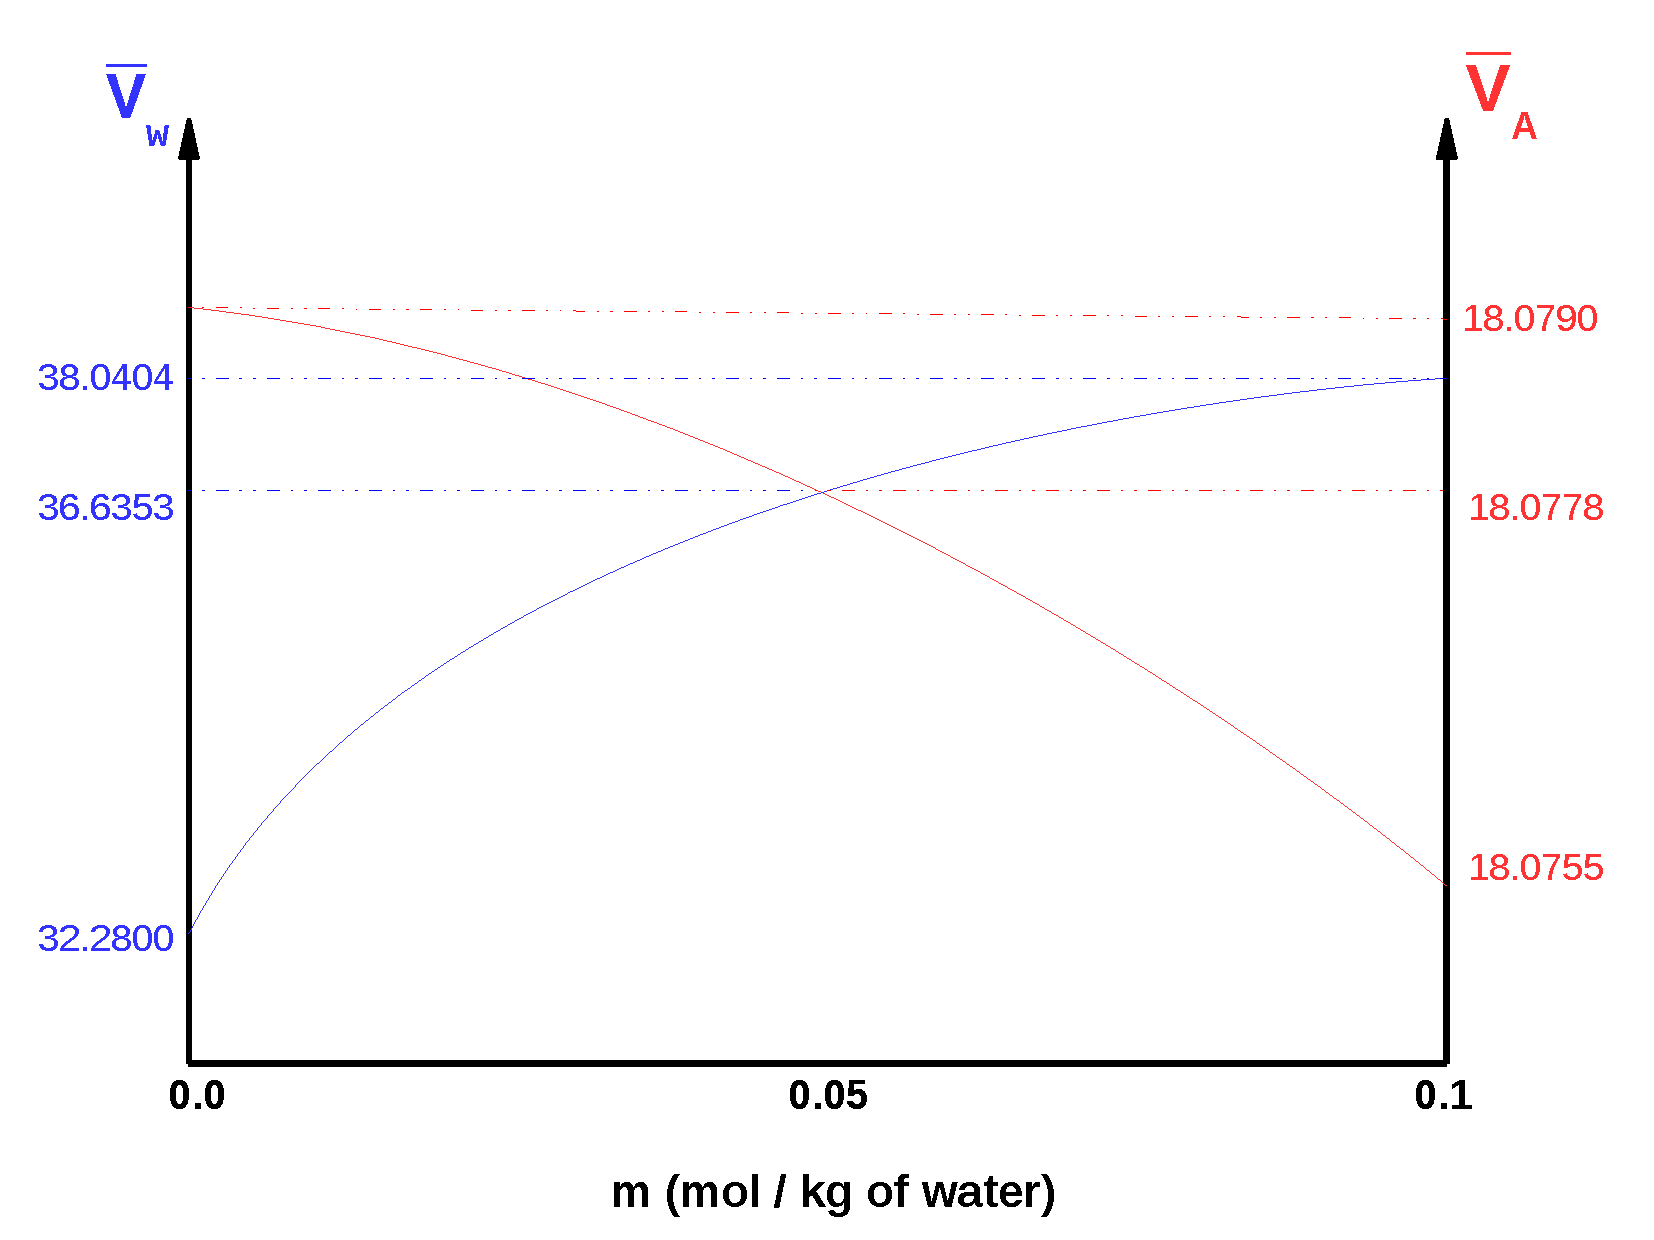
\includegraphics[width=0.75\columnwidth,clip]{./../Pics/Example04_Pic}
          \end{center}
\end{itemize}


\clearpage
            
%%%
%%% EXAMPLE:  NPTEl (Ex 6.3)
%%%
   \item\label{Mod05Ex06} What is the change in entropy when 0.6 m$^{3}$ of CO$_{2}$ and 0.4 m$^{3}$ of N$_{2}$, each at 1 bar and 25 $^{\circ}$C blend to form a gas mixture at the same conditions. Assume ideal gas behaviour and that {\it mole fraction = volume fraction}. 

% SOLUTION
       \noindent{\bf Solution:} For an ideal gas, with the assumption of {\it mole fraction = volume fraction}, \ie $y_{1} = 0.6$ and $y_{2} = 0.4$, with CO$_{2}$:1 and N$_{2}$:2.
      \begin{displaymath}
          \Delta_{\text{mix}}\overline{s}^{\text{igm}} = -R\summation[y_{i}\ln{y_{i}}]{i=1}{2} = 5.5954 \text{ J.(mol.K)}^{-1}
      \end{displaymath}


\clearpage
            
%%%
%%% EXAMPLE:  SM&VN 10.20 (pg 350)
%%%
   \item\label{Mod05Ex07}  For the acetone (Ket) / methanol (MetOH) system, a vapour mixture of $z_{\text{Ket}}$ = 0.25 and $z_{\text{MetOH}}$ = 0.75 is cooled to temperature $T$ in the two-phase region and flows into a separation chamber at a pressure of 1 bar. If the composition of the liquid product is $x_{\text{Ket}}$ = 0.175, calculate $T$  and $y_{\text{Ket}}$. For liquid mixture, assume that
\begin{displaymath}
\ln\gamma_{1} = 0.64x_{2}^{2} \;\;\;\;\;\text{ and }\;\;\;\;\;\ln\gamma_{2}=0.64x_{1}^{2}
\end{displaymath}
For the Antoine equation, 
\begin{displaymath}
\ln P_{i}^{\text{sat}} = A_{i} - \frc{B_{i}}{T + C} \;\;\left(\text{ [P] = kPa and [T] = }^{\circ}\text{C}\right)
\end{displaymath}
$A_{\text{Ket}}$ = 14.3145, $B_{\text{Ket}}$ = 2756.22$^{\circ}$C, $C_{\text{Ket}}$ = 228.060$^{\circ}$C, $A_{\text{MetOH}}$ = 16.5785, $B_{\text{MetOH}}$ = 3638.27$^{\circ}$C, $C_{\text{MetOH}}$ = 239.50$^{\circ}$C.

% SOLUTION
       \noindent{\bf Solution:} This is a typical flash problem for separation of acetone (1) and methanol (2). The feed stream contains 25$\%$-mol of acetone, \ie $z_{1}=0.25$, and after the separation at 1 bar, the resulting liquid stream contains 17.5$\%$-mol, \ie $x_{1}=0.175$. The problem requires temperature of the separation and composition of the gas stream, $y_{i}$. As $\gamma_{i}$ is given, we can consider that the liquid mixture is {\bf not ideal}, therefore the modified Raoult's law can be used,
\begin{displaymath}
    y_{i}P = x_{i}\gamma_{i}P_{i}^{\text{sat}} \;\;\;\longrightarrow y_{1}=\frc{x_{1}\gamma_{1}P_{1}^{\text{sat}}}{P}
\end{displaymath}
    
  \begin{figure}[h]
     \begin{center}
         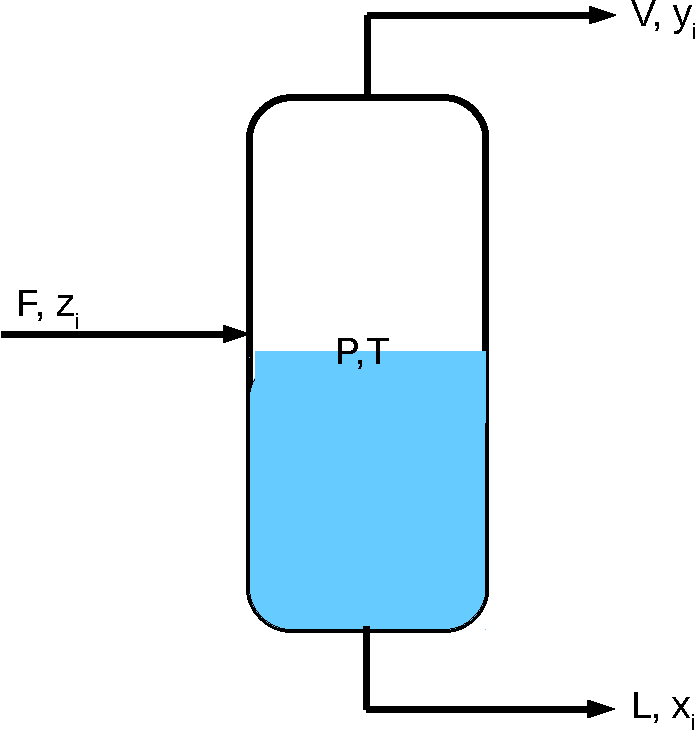
\includegraphics[width=.25\linewidth,clip]{./Figs/FlashDistillation}
     \end{center}
     \caption{Schematic of a flash process, Example~\ref{Mod05Ex07}.}
  \end{figure}

 Using the material balance derived in Section~\ref{Section:04:FlashDistillation},
\begin{eqnarray}
    && Fz_{1} = x_{1}L + y_{1}V\;\;\text{ and for } \;F=1\;\text{ (\ie normalised stream fractions)}\;\;\;\longrightarrow F = L + V = 1,\text{ leading to} \nonumber \\
    && z_{1} = x_{1}L + \frc{x_{1}\gamma_{1}P_{1}^{\text{sat}}}{p}\left(1-L\right)\;(\star)\;\; \text{ with }\;\; P=\summation[P_{i}]{i}{} = y_{1}P + y_{2}P = x_{1}\gamma_{1}P_{1}^{\text{sat}} + x_{2}\gamma_{2}P_{2}^{\text{sat}}\;(\dagger),\nonumber
\end{eqnarray}
therefore, we have 2 equations and 2 unknowns, $L$ and $T$. Let's solve ($\dagger$) first for $T$ with $\gamma_{1}=1.5459$ and $\gamma_{2}=1.0198$
   \begin{displaymath}
       P = x_{1}\gamma_{1}P_{1}^{\text{sat}} + x_{2}\gamma_{2}P_{2}^{\text{sat}} = 100 \text{ kPa} \;\;\;\Rightarrow\;\;\; T = 59.5309\text{ K}
   \end{displaymath}
 With $T$, we can solve ($\star$) for $L$,
   \begin{eqnarray}
       && z_{1} = x_{1}L + \frc{x_{1}\gamma_{1}P_{1}^{\text{sat}}}{p}\left(1-L\right) \nonumber \\
       && L = \frc{z_{1} - \frac{x_{1}\gamma_{1}P_{1}^{\text{sat}}}{P}}{x_{1} - \frac{x_{1}\gamma_{1}P_{1}^{\text{sat}}}{P}} = 0.4306\;\;\rightarrow \;\; V = 0.5694 \nonumber \\
       && y_{1} = \frac{x_{1}\gamma_{1}P_{1}^{\text{sat}}}{P} = 0.3067\;\;\rightarrow \;\; y_{2} = 0.6933\nonumber
   \end{eqnarray}
 



\end{enumerate}
